\documentclass[twoside]{book}

% Packages required by doxygen
\usepackage{fixltx2e}
\usepackage{calc}
\usepackage{doxygen}
\usepackage[export]{adjustbox} % also loads graphicx
\usepackage{graphicx}
\usepackage[utf8]{inputenc}
\usepackage{makeidx}
\usepackage{multicol}
\usepackage{multirow}
\PassOptionsToPackage{warn}{textcomp}
\usepackage{textcomp}
\usepackage[nointegrals]{wasysym}
\usepackage[table]{xcolor}

% Font selection
\usepackage[T1]{fontenc}
\usepackage[scaled=.90]{helvet}
\usepackage{courier}
\usepackage{amssymb}
\usepackage{sectsty}
\renewcommand{\familydefault}{\sfdefault}
\allsectionsfont{%
  \fontseries{bc}\selectfont%
  \color{darkgray}%
}
\renewcommand{\DoxyLabelFont}{%
  \fontseries{bc}\selectfont%
  \color{darkgray}%
}
\newcommand{\+}{\discretionary{\mbox{\scriptsize$\hookleftarrow$}}{}{}}

% Page & text layout
\usepackage{geometry}
\geometry{%
  a4paper,%
  top=2.5cm,%
  bottom=2.5cm,%
  left=2.5cm,%
  right=2.5cm%
}
\tolerance=750
\hfuzz=15pt
\hbadness=750
\setlength{\emergencystretch}{15pt}
\setlength{\parindent}{0cm}
\setlength{\parskip}{0.2cm}
\makeatletter
\renewcommand{\paragraph}{%
  \@startsection{paragraph}{4}{0ex}{-1.0ex}{1.0ex}{%
    \normalfont\normalsize\bfseries\SS@parafont%
  }%
}
\renewcommand{\subparagraph}{%
  \@startsection{subparagraph}{5}{0ex}{-1.0ex}{1.0ex}{%
    \normalfont\normalsize\bfseries\SS@subparafont%
  }%
}
\makeatother

% Headers & footers
\usepackage{fancyhdr}
\pagestyle{fancyplain}
\fancyhead[LE]{\fancyplain{}{\bfseries\thepage}}
\fancyhead[CE]{\fancyplain{}{}}
\fancyhead[RE]{\fancyplain{}{\bfseries\leftmark}}
\fancyhead[LO]{\fancyplain{}{\bfseries\rightmark}}
\fancyhead[CO]{\fancyplain{}{}}
\fancyhead[RO]{\fancyplain{}{\bfseries\thepage}}
\fancyfoot[LE]{\fancyplain{}{}}
\fancyfoot[CE]{\fancyplain{}{}}
\fancyfoot[RE]{\fancyplain{}{\bfseries\scriptsize Generated on Thu Feb 25 2016 05\+:26\+:37 for Rollo -\/ Localization of a humanoid robot by Doxygen }}
\fancyfoot[LO]{\fancyplain{}{\bfseries\scriptsize Generated on Thu Feb 25 2016 05\+:26\+:37 for Rollo -\/ Localization of a humanoid robot by Doxygen }}
\fancyfoot[CO]{\fancyplain{}{}}
\fancyfoot[RO]{\fancyplain{}{}}
\renewcommand{\footrulewidth}{0.4pt}
\renewcommand{\chaptermark}[1]{%
  \markboth{#1}{}%
}
\renewcommand{\sectionmark}[1]{%
  \markright{\thesection\ #1}%
}

% Indices & bibliography
\usepackage{natbib}
\usepackage[titles]{tocloft}
\setcounter{tocdepth}{3}
\setcounter{secnumdepth}{5}
\makeindex

% Hyperlinks (required, but should be loaded last)
\usepackage{ifpdf}
\ifpdf
  \usepackage[pdftex,pagebackref=true]{hyperref}
\else
  \usepackage[ps2pdf,pagebackref=true]{hyperref}
\fi
\hypersetup{%
  colorlinks=true,%
  linkcolor=blue,%
  citecolor=blue,%
  unicode%
}

% Custom commands
\newcommand{\clearemptydoublepage}{%
  \newpage{\pagestyle{empty}\cleardoublepage}%
}


%===== C O N T E N T S =====

\begin{document}

% Titlepage & ToC
\hypersetup{pageanchor=false,
             bookmarks=true,
             bookmarksnumbered=true,
             pdfencoding=unicode
            }
\pagenumbering{roman}
\begin{titlepage}
\vspace*{7cm}
\begin{center}%
{\Large Rollo -\/ Localization of a humanoid robot \\[1ex]\large 1.\+0 }\\
\vspace*{1cm}
{\large Generated by Doxygen 1.8.10}\\
\vspace*{0.5cm}
{\small Thu Feb 25 2016 05:26:37}\\
\end{center}
\end{titlepage}
\clearemptydoublepage
\tableofcontents
\clearemptydoublepage
\pagenumbering{arabic}
\hypersetup{pageanchor=true}

%--- Begin generated contents ---
\chapter{Hierarchical Index}
\section{Class Hierarchy}
This inheritance list is sorted roughly, but not completely, alphabetically\+:\begin{DoxyCompactList}
\item runtime\+\_\+error\begin{DoxyCompactList}
\item \contentsline{section}{udp\+\_\+client\+\_\+server\+:\+:udp\+\_\+client\+\_\+server\+\_\+runtime\+\_\+error}{\pageref{classudp__client__server_1_1udp__client__server__runtime__error}}{}
\end{DoxyCompactList}
\item \contentsline{section}{udp\+\_\+client\+\_\+server\+:\+:udp\+\_\+client}{\pageref{classudp__client__server_1_1udp__client}}{}
\item \contentsline{section}{udp\+\_\+client\+\_\+server\+:\+:udp\+\_\+server}{\pageref{classudp__client__server_1_1udp__server}}{}
\end{DoxyCompactList}

\chapter{Class Index}
\section{Class List}
Here are the classes, structs, unions and interfaces with brief descriptions\+:\begin{DoxyCompactList}
\item\contentsline{section}{\hyperlink{classudp__client__server_1_1udp__client}{udp\+\_\+client\+\_\+server\+::udp\+\_\+client} }{\pageref{classudp__client__server_1_1udp__client}}{}
\item\contentsline{section}{\hyperlink{classudp__client__server_1_1udp__client__server__runtime__error}{udp\+\_\+client\+\_\+server\+::udp\+\_\+client\+\_\+server\+\_\+runtime\+\_\+error} }{\pageref{classudp__client__server_1_1udp__client__server__runtime__error}}{}
\item\contentsline{section}{\hyperlink{classudp__client__server_1_1udp__server}{udp\+\_\+client\+\_\+server\+::udp\+\_\+server} }{\pageref{classudp__client__server_1_1udp__server}}{}
\end{DoxyCompactList}

\chapter{File Index}
\section{File List}
Here is a list of all documented files with brief descriptions\+:\begin{DoxyCompactList}
\item\contentsline{section}{/home/emeres/.\+hdd/\+Documents/\+Studia/\+Università degli studi di Genova/\+D\+I\+B\+R\+I\+S/\+Tutti i corsi/86805 -\/ S\+O\+F\+T\+W\+A\+R\+E A\+R\+C\+H\+I\+T\+E\+C\+T\+U\+R\+E\+S F\+O\+R R\+O\+B\+O\+T\+I\+C\+S/\+A\+S01/rollo/src/\hyperlink{rollo_8hpp}{rollo.\+hpp} \\*Header file holding Rollo specific parameters and global references for the R\+O\+S nodes }{\pageref{rollo_8hpp}}{}
\item\contentsline{section}{/home/emeres/.\+hdd/\+Documents/\+Studia/\+Università degli studi di Genova/\+D\+I\+B\+R\+I\+S/\+Tutti i corsi/86805 -\/ S\+O\+F\+T\+W\+A\+R\+E A\+R\+C\+H\+I\+T\+E\+C\+T\+U\+R\+E\+S F\+O\+R R\+O\+B\+O\+T\+I\+C\+S/\+A\+S01/rollo/src/\hyperlink{rollo__comm_8cpp}{rollo\+\_\+comm.\+cpp} \\*Communication between R\+O\+S and Rollo }{\pageref{rollo__comm_8cpp}}{}
\item\contentsline{section}{/home/emeres/.\+hdd/\+Documents/\+Studia/\+Università degli studi di Genova/\+D\+I\+B\+R\+I\+S/\+Tutti i corsi/86805 -\/ S\+O\+F\+T\+W\+A\+R\+E A\+R\+C\+H\+I\+T\+E\+C\+T\+U\+R\+E\+S F\+O\+R R\+O\+B\+O\+T\+I\+C\+S/\+A\+S01/rollo/src/\hyperlink{rollo__control_8cpp}{rollo\+\_\+control.\+cpp} \\*Takes input from keyboard and publishes commands to control Rollo }{\pageref{rollo__control_8cpp}}{}
\item\contentsline{section}{/home/emeres/.\+hdd/\+Documents/\+Studia/\+Università degli studi di Genova/\+D\+I\+B\+R\+I\+S/\+Tutti i corsi/86805 -\/ S\+O\+F\+T\+W\+A\+R\+E A\+R\+C\+H\+I\+T\+E\+C\+T\+U\+R\+E\+S F\+O\+R R\+O\+B\+O\+T\+I\+C\+S/\+A\+S01/rollo/src/\hyperlink{rollo__ekf_8cpp}{rollo\+\_\+ekf.\+cpp} \\*E\+K\+F implementation for localisation of the robot }{\pageref{rollo__ekf_8cpp}}{}
\item\contentsline{section}{/home/emeres/.\+hdd/\+Documents/\+Studia/\+Università degli studi di Genova/\+D\+I\+B\+R\+I\+S/\+Tutti i corsi/86805 -\/ S\+O\+F\+T\+W\+A\+R\+E A\+R\+C\+H\+I\+T\+E\+C\+T\+U\+R\+E\+S F\+O\+R R\+O\+B\+O\+T\+I\+C\+S/\+A\+S01/rollo/src/{\bfseries udp.\+h} }{\pageref{udp_8h}}{}
\end{DoxyCompactList}

\chapter{Class Documentation}
\hypertarget{classudp__client__server_1_1udp__client}{}\section{udp\+\_\+client\+\_\+server\+:\+:udp\+\_\+client Class Reference}
\label{classudp__client__server_1_1udp__client}\index{udp\+\_\+client\+\_\+server\+::udp\+\_\+client@{udp\+\_\+client\+\_\+server\+::udp\+\_\+client}}
\subsection*{Public Member Functions}
\begin{DoxyCompactItemize}
\item 
\hyperlink{classudp__client__server_1_1udp__client_a2d019e5e93a971262f3ee4476be0427a}{udp\+\_\+client} (const std\+::string \&addr, int \hyperlink{rollo__comm_8cpp_a63c89c04d1feae07ca35558055155ffb}{port})
\begin{DoxyCompactList}\small\item\em Initialize a U\+D\+P client object. \end{DoxyCompactList}\item 
\hyperlink{classudp__client__server_1_1udp__client_a2d86924b0df64eaa14db80ece0ab7812}{$\sim$udp\+\_\+client} ()
\begin{DoxyCompactList}\small\item\em Clean up the U\+D\+P client object. \end{DoxyCompactList}\item 
int \hyperlink{classudp__client__server_1_1udp__client_adb58b691a3fb90f86d6643e01123d528}{get\+\_\+socket} () const 
\begin{DoxyCompactList}\small\item\em Retrieve a copy of the socket identifier. \end{DoxyCompactList}\item 
int \hyperlink{classudp__client__server_1_1udp__client_ab4d8fc06bab9b1ab1435fa9d9a7bd9f8}{get\+\_\+port} () const 
\begin{DoxyCompactList}\small\item\em Retrieve the port used by this U\+D\+P client. \end{DoxyCompactList}\item 
std\+::string \hyperlink{classudp__client__server_1_1udp__client_a1fbf29e1facd0a802a5032aa0273af63}{get\+\_\+addr} () const 
\begin{DoxyCompactList}\small\item\em Retrieve a copy of the address. \end{DoxyCompactList}\item 
int \hyperlink{classudp__client__server_1_1udp__client_ac296d1fb6a6006bec5f8f14a81367d0a}{send} (const char $\ast$msg, size\+\_\+t size)
\begin{DoxyCompactList}\small\item\em Send a message through this U\+D\+P client. \end{DoxyCompactList}\end{DoxyCompactItemize}


\subsection{Constructor \& Destructor Documentation}
\hypertarget{classudp__client__server_1_1udp__client_a2d019e5e93a971262f3ee4476be0427a}{}\index{udp\+\_\+client\+\_\+server\+::udp\+\_\+client@{udp\+\_\+client\+\_\+server\+::udp\+\_\+client}!udp\+\_\+client@{udp\+\_\+client}}
\index{udp\+\_\+client@{udp\+\_\+client}!udp\+\_\+client\+\_\+server\+::udp\+\_\+client@{udp\+\_\+client\+\_\+server\+::udp\+\_\+client}}
\subsubsection[{udp\+\_\+client(const std\+::string \&addr, int port)}]{\setlength{\rightskip}{0pt plus 5cm}udp\+\_\+client\+\_\+server\+::udp\+\_\+client\+::udp\+\_\+client (
\begin{DoxyParamCaption}
\item[{const std\+::string \&}]{addr, }
\item[{int}]{port}
\end{DoxyParamCaption}
)}\label{classudp__client__server_1_1udp__client_a2d019e5e93a971262f3ee4476be0427a}


Initialize a U\+D\+P client object. 

This function initializes the U\+D\+P client object using the address and the port as specified.

The port is expected to be a host side port number (i.\+e. 59200).

The {\ttfamily addr} parameter is a textual address. It may be an I\+Pv4 or I\+Pv6 address and it can represent a host name or an address defined with just numbers. If the address cannot be resolved then an error occurs and constructor throws.

\begin{DoxyNote}{Note}
The socket is open in this process. If you fork() or exec() then the socket will be closed by the operating system.
\end{DoxyNote}
\begin{DoxyWarning}{Warning}
We only make use of the first address found by getaddrinfo(). All the other addresses are ignored.
\end{DoxyWarning}

\begin{DoxyExceptions}{Exceptions}
{\em \hyperlink{classudp__client__server_1_1udp__client__server__runtime__error}{udp\+\_\+client\+\_\+server\+\_\+runtime\+\_\+error}} & The server could not be initialized properly. Either the address cannot be resolved, the port is incompatible or not available, or the socket could not be created.\\
\hline
\end{DoxyExceptions}

\begin{DoxyParams}[1]{Parameters}
\mbox{\tt in}  & {\em addr} & The address to convert to a numeric I\+P. \\
\hline
\mbox{\tt in}  & {\em port} & The port number. \\
\hline
\end{DoxyParams}
\hypertarget{classudp__client__server_1_1udp__client_a2d86924b0df64eaa14db80ece0ab7812}{}\index{udp\+\_\+client\+\_\+server\+::udp\+\_\+client@{udp\+\_\+client\+\_\+server\+::udp\+\_\+client}!````~udp\+\_\+client@{$\sim$udp\+\_\+client}}
\index{````~udp\+\_\+client@{$\sim$udp\+\_\+client}!udp\+\_\+client\+\_\+server\+::udp\+\_\+client@{udp\+\_\+client\+\_\+server\+::udp\+\_\+client}}
\subsubsection[{$\sim$udp\+\_\+client()}]{\setlength{\rightskip}{0pt plus 5cm}udp\+\_\+client\+\_\+server\+::udp\+\_\+client\+::$\sim$udp\+\_\+client (
\begin{DoxyParamCaption}
{}
\end{DoxyParamCaption}
)}\label{classudp__client__server_1_1udp__client_a2d86924b0df64eaa14db80ece0ab7812}


Clean up the U\+D\+P client object. 

This function frees the address information structure and close the socket before returning. 

\subsection{Member Function Documentation}
\hypertarget{classudp__client__server_1_1udp__client_a1fbf29e1facd0a802a5032aa0273af63}{}\index{udp\+\_\+client\+\_\+server\+::udp\+\_\+client@{udp\+\_\+client\+\_\+server\+::udp\+\_\+client}!get\+\_\+addr@{get\+\_\+addr}}
\index{get\+\_\+addr@{get\+\_\+addr}!udp\+\_\+client\+\_\+server\+::udp\+\_\+client@{udp\+\_\+client\+\_\+server\+::udp\+\_\+client}}
\subsubsection[{get\+\_\+addr() const }]{\setlength{\rightskip}{0pt plus 5cm}std\+::string udp\+\_\+client\+\_\+server\+::udp\+\_\+client\+::get\+\_\+addr (
\begin{DoxyParamCaption}
{}
\end{DoxyParamCaption}
) const}\label{classudp__client__server_1_1udp__client_a1fbf29e1facd0a802a5032aa0273af63}


Retrieve a copy of the address. 

This function returns a copy of the address as it was specified in the constructor. This does not return a canonalized version of the address.

The address cannot be modified. If you need to send data on a different address, create a new U\+D\+P client.

\begin{DoxyReturn}{Returns}
A string with a copy of the constructor input address. 
\end{DoxyReturn}
\hypertarget{classudp__client__server_1_1udp__client_ab4d8fc06bab9b1ab1435fa9d9a7bd9f8}{}\index{udp\+\_\+client\+\_\+server\+::udp\+\_\+client@{udp\+\_\+client\+\_\+server\+::udp\+\_\+client}!get\+\_\+port@{get\+\_\+port}}
\index{get\+\_\+port@{get\+\_\+port}!udp\+\_\+client\+\_\+server\+::udp\+\_\+client@{udp\+\_\+client\+\_\+server\+::udp\+\_\+client}}
\subsubsection[{get\+\_\+port() const }]{\setlength{\rightskip}{0pt plus 5cm}int udp\+\_\+client\+\_\+server\+::udp\+\_\+client\+::get\+\_\+port (
\begin{DoxyParamCaption}
{}
\end{DoxyParamCaption}
) const}\label{classudp__client__server_1_1udp__client_ab4d8fc06bab9b1ab1435fa9d9a7bd9f8}


Retrieve the port used by this U\+D\+P client. 

This function returns the port used by this U\+D\+P client. The port is defined as an integer, host side.

\begin{DoxyReturn}{Returns}
The port as expected in a host integer. 
\end{DoxyReturn}
\hypertarget{classudp__client__server_1_1udp__client_adb58b691a3fb90f86d6643e01123d528}{}\index{udp\+\_\+client\+\_\+server\+::udp\+\_\+client@{udp\+\_\+client\+\_\+server\+::udp\+\_\+client}!get\+\_\+socket@{get\+\_\+socket}}
\index{get\+\_\+socket@{get\+\_\+socket}!udp\+\_\+client\+\_\+server\+::udp\+\_\+client@{udp\+\_\+client\+\_\+server\+::udp\+\_\+client}}
\subsubsection[{get\+\_\+socket() const }]{\setlength{\rightskip}{0pt plus 5cm}int udp\+\_\+client\+\_\+server\+::udp\+\_\+client\+::get\+\_\+socket (
\begin{DoxyParamCaption}
{}
\end{DoxyParamCaption}
) const}\label{classudp__client__server_1_1udp__client_adb58b691a3fb90f86d6643e01123d528}


Retrieve a copy of the socket identifier. 

This function return the socket identifier as returned by the socket() function. This can be used to change some flags.

\begin{DoxyReturn}{Returns}
The socket used by this U\+D\+P client. 
\end{DoxyReturn}
\hypertarget{classudp__client__server_1_1udp__client_ac296d1fb6a6006bec5f8f14a81367d0a}{}\index{udp\+\_\+client\+\_\+server\+::udp\+\_\+client@{udp\+\_\+client\+\_\+server\+::udp\+\_\+client}!send@{send}}
\index{send@{send}!udp\+\_\+client\+\_\+server\+::udp\+\_\+client@{udp\+\_\+client\+\_\+server\+::udp\+\_\+client}}
\subsubsection[{send(const char $\ast$msg, size\+\_\+t size)}]{\setlength{\rightskip}{0pt plus 5cm}int udp\+\_\+client\+\_\+server\+::udp\+\_\+client\+::send (
\begin{DoxyParamCaption}
\item[{const char $\ast$}]{msg, }
\item[{size\+\_\+t}]{size}
\end{DoxyParamCaption}
)}\label{classudp__client__server_1_1udp__client_ac296d1fb6a6006bec5f8f14a81367d0a}


Send a message through this U\+D\+P client. 

This function sends {\ttfamily msg} through the U\+D\+P client socket. The function cannot be used to change the destination as it was defined when creating the \hyperlink{classudp__client__server_1_1udp__client}{udp\+\_\+client} object.

The size must be small enough for the message to fit. In most cases we use these in Snap! to send very small signals (i.\+e. 4 bytes commands.) Any data we would want to share remains in the Cassandra database so that way we can avoid losing it because of a U\+D\+P message.


\begin{DoxyParams}[1]{Parameters}
\mbox{\tt in}  & {\em msg} & The message to send. \\
\hline
\mbox{\tt in}  & {\em size} & The number of bytes representing this message.\\
\hline
\end{DoxyParams}
\begin{DoxyReturn}{Returns}
-\/1 if an error occurs, otherwise the number of bytes sent. errno is set accordingly on error. 
\end{DoxyReturn}


The documentation for this class was generated from the following files\+:\begin{DoxyCompactItemize}
\item 
/home/emeres/.\+hdd/\+Documents/\+Studia/\+Università degli studi di Genova/\+D\+I\+B\+R\+I\+S/\+Tutti i corsi/86805 -\/ S\+O\+F\+T\+W\+A\+R\+E A\+R\+C\+H\+I\+T\+E\+C\+T\+U\+R\+E\+S F\+O\+R R\+O\+B\+O\+T\+I\+C\+S/\+A\+S01/rollo/src/udp.\+h\item 
/home/emeres/.\+hdd/\+Documents/\+Studia/\+Università degli studi di Genova/\+D\+I\+B\+R\+I\+S/\+Tutti i corsi/86805 -\/ S\+O\+F\+T\+W\+A\+R\+E A\+R\+C\+H\+I\+T\+E\+C\+T\+U\+R\+E\+S F\+O\+R R\+O\+B\+O\+T\+I\+C\+S/\+A\+S01/rollo/src/udp.\+cpp\end{DoxyCompactItemize}

\hypertarget{classudp__client__server_1_1udp__client__server__runtime__error}{}\section{udp\+\_\+client\+\_\+server\+:\+:udp\+\_\+client\+\_\+server\+\_\+runtime\+\_\+error Class Reference}
\label{classudp__client__server_1_1udp__client__server__runtime__error}\index{udp\+\_\+client\+\_\+server\+::udp\+\_\+client\+\_\+server\+\_\+runtime\+\_\+error@{udp\+\_\+client\+\_\+server\+::udp\+\_\+client\+\_\+server\+\_\+runtime\+\_\+error}}
Inheritance diagram for udp\+\_\+client\+\_\+server\+:\+:udp\+\_\+client\+\_\+server\+\_\+runtime\+\_\+error\+:\begin{figure}[H]
\begin{center}
\leavevmode
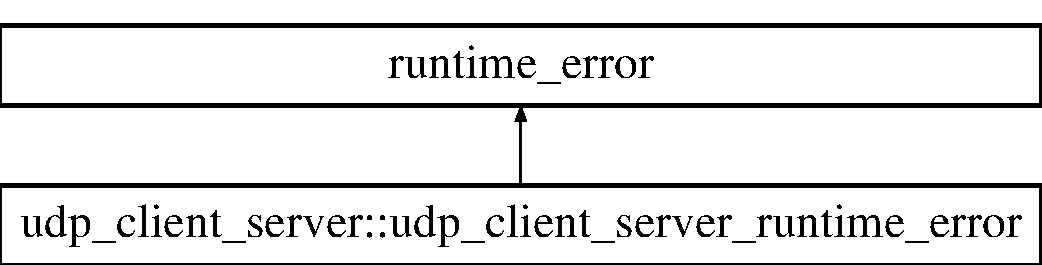
\includegraphics[height=2.000000cm]{classudp__client__server_1_1udp__client__server__runtime__error}
\end{center}
\end{figure}
\subsection*{Public Member Functions}
\begin{DoxyCompactItemize}
\item 
\hypertarget{classudp__client__server_1_1udp__client__server__runtime__error_add3731a02166e43ef92ba4e031e046c6}{}{\bfseries udp\+\_\+client\+\_\+server\+\_\+runtime\+\_\+error} (const char $\ast$w)\label{classudp__client__server_1_1udp__client__server__runtime__error_add3731a02166e43ef92ba4e031e046c6}

\end{DoxyCompactItemize}


The documentation for this class was generated from the following file\+:\begin{DoxyCompactItemize}
\item 
/home/emeres/.\+hdd/\+Documents/\+Studia/\+Università degli studi di Genova/\+D\+I\+B\+R\+I\+S/\+Tutti i corsi/86805 -\/ S\+O\+F\+T\+W\+A\+R\+E A\+R\+C\+H\+I\+T\+E\+C\+T\+U\+R\+E\+S F\+O\+R R\+O\+B\+O\+T\+I\+C\+S/\+A\+S01/rollo/src/udp.\+h\end{DoxyCompactItemize}

\hypertarget{classudp__client__server_1_1udp__server}{}\section{udp\+\_\+client\+\_\+server\+:\+:udp\+\_\+server Class Reference}
\label{classudp__client__server_1_1udp__server}\index{udp\+\_\+client\+\_\+server\+::udp\+\_\+server@{udp\+\_\+client\+\_\+server\+::udp\+\_\+server}}
\subsection*{Public Member Functions}
\begin{DoxyCompactItemize}
\item 
\hyperlink{classudp__client__server_1_1udp__server_ae44891f41370ca856da0fe50923a1b25}{udp\+\_\+server} (const std\+::string \&addr, int \hyperlink{rollo__comm_8cpp_a63c89c04d1feae07ca35558055155ffb}{port})
\begin{DoxyCompactList}\small\item\em Initialize a U\+D\+P server object. \end{DoxyCompactList}\item 
\hyperlink{classudp__client__server_1_1udp__server_acdce04ccdcc420d4f959110c75ec9b1c}{$\sim$udp\+\_\+server} ()
\begin{DoxyCompactList}\small\item\em Clean up the U\+D\+P server. \end{DoxyCompactList}\item 
int \hyperlink{classudp__client__server_1_1udp__server_ace51743964b568c021b0f3154f4c0306}{get\+\_\+socket} () const 
\begin{DoxyCompactList}\small\item\em The socket used by this U\+D\+P server. \end{DoxyCompactList}\item 
int \hyperlink{classudp__client__server_1_1udp__server_a78b6867c5dc04599c8b146fe4971459a}{get\+\_\+port} () const 
\begin{DoxyCompactList}\small\item\em The port used by this U\+D\+P server. \end{DoxyCompactList}\item 
std\+::string \hyperlink{classudp__client__server_1_1udp__server_a9b82191caf4ccc1d6822d5f92e382e02}{get\+\_\+addr} () const 
\begin{DoxyCompactList}\small\item\em Return the address of this U\+D\+P server. \end{DoxyCompactList}\item 
int \hyperlink{classudp__client__server_1_1udp__server_aa103886a58d575868dc01ad0d3f73cbc}{recv} (char $\ast$msg, size\+\_\+t max\+\_\+size)
\begin{DoxyCompactList}\small\item\em Wait on a message. \end{DoxyCompactList}\item 
int \hyperlink{classudp__client__server_1_1udp__server_af376121a83f6c07187f077bc77aa6e27}{timed\+\_\+recv} (char $\ast$msg, size\+\_\+t max\+\_\+size, int max\+\_\+wait\+\_\+ms)
\begin{DoxyCompactList}\small\item\em Wait for data to come in. \end{DoxyCompactList}\end{DoxyCompactItemize}


\subsection{Constructor \& Destructor Documentation}
\hypertarget{classudp__client__server_1_1udp__server_ae44891f41370ca856da0fe50923a1b25}{}\index{udp\+\_\+client\+\_\+server\+::udp\+\_\+server@{udp\+\_\+client\+\_\+server\+::udp\+\_\+server}!udp\+\_\+server@{udp\+\_\+server}}
\index{udp\+\_\+server@{udp\+\_\+server}!udp\+\_\+client\+\_\+server\+::udp\+\_\+server@{udp\+\_\+client\+\_\+server\+::udp\+\_\+server}}
\subsubsection[{udp\+\_\+server(const std\+::string \&addr, int port)}]{\setlength{\rightskip}{0pt plus 5cm}udp\+\_\+client\+\_\+server\+::udp\+\_\+server\+::udp\+\_\+server (
\begin{DoxyParamCaption}
\item[{const std\+::string \&}]{addr, }
\item[{int}]{port}
\end{DoxyParamCaption}
)}\label{classudp__client__server_1_1udp__server_ae44891f41370ca856da0fe50923a1b25}


Initialize a U\+D\+P server object. 

This function initializes a U\+D\+P server object making it ready to receive messages.

The server address and port are specified in the constructor so if you need to receive messages from several different addresses and/or port, you\textquotesingle{}ll have to create a server for each.

The address is a string and it can represent an I\+Pv4 or I\+Pv6 address.

Note that this function calls connect() to connect the socket to the specified address. To accept data on different U\+D\+P addresses and ports, multiple U\+D\+P servers must be created.

\begin{DoxyNote}{Note}
The socket is open in this process. If you fork() or exec() then the socket will be closed by the operating system.
\end{DoxyNote}
\begin{DoxyWarning}{Warning}
We only make use of the first address found by getaddrinfo(). All the other addresses are ignored.
\end{DoxyWarning}

\begin{DoxyExceptions}{Exceptions}
{\em \hyperlink{classudp__client__server_1_1udp__client__server__runtime__error}{udp\+\_\+client\+\_\+server\+\_\+runtime\+\_\+error}} & The \hyperlink{classudp__client__server_1_1udp__client__server__runtime__error}{udp\+\_\+client\+\_\+server\+\_\+runtime\+\_\+error} exception is raised when the address and port combinaison cannot be resolved or if the socket cannot be opened.\\
\hline
\end{DoxyExceptions}

\begin{DoxyParams}[1]{Parameters}
\mbox{\tt in}  & {\em addr} & The address we receive on. \\
\hline
\mbox{\tt in}  & {\em port} & The port we receive from. \\
\hline
\end{DoxyParams}
\hypertarget{classudp__client__server_1_1udp__server_acdce04ccdcc420d4f959110c75ec9b1c}{}\index{udp\+\_\+client\+\_\+server\+::udp\+\_\+server@{udp\+\_\+client\+\_\+server\+::udp\+\_\+server}!````~udp\+\_\+server@{$\sim$udp\+\_\+server}}
\index{````~udp\+\_\+server@{$\sim$udp\+\_\+server}!udp\+\_\+client\+\_\+server\+::udp\+\_\+server@{udp\+\_\+client\+\_\+server\+::udp\+\_\+server}}
\subsubsection[{$\sim$udp\+\_\+server()}]{\setlength{\rightskip}{0pt plus 5cm}udp\+\_\+client\+\_\+server\+::udp\+\_\+server\+::$\sim$udp\+\_\+server (
\begin{DoxyParamCaption}
{}
\end{DoxyParamCaption}
)}\label{classudp__client__server_1_1udp__server_acdce04ccdcc420d4f959110c75ec9b1c}


Clean up the U\+D\+P server. 

This function frees the address info structures and close the socket. 

\subsection{Member Function Documentation}
\hypertarget{classudp__client__server_1_1udp__server_a9b82191caf4ccc1d6822d5f92e382e02}{}\index{udp\+\_\+client\+\_\+server\+::udp\+\_\+server@{udp\+\_\+client\+\_\+server\+::udp\+\_\+server}!get\+\_\+addr@{get\+\_\+addr}}
\index{get\+\_\+addr@{get\+\_\+addr}!udp\+\_\+client\+\_\+server\+::udp\+\_\+server@{udp\+\_\+client\+\_\+server\+::udp\+\_\+server}}
\subsubsection[{get\+\_\+addr() const }]{\setlength{\rightskip}{0pt plus 5cm}std\+::string udp\+\_\+client\+\_\+server\+::udp\+\_\+server\+::get\+\_\+addr (
\begin{DoxyParamCaption}
{}
\end{DoxyParamCaption}
) const}\label{classudp__client__server_1_1udp__server_a9b82191caf4ccc1d6822d5f92e382e02}


Return the address of this U\+D\+P server. 

This function returns a verbatim copy of the address as passed to the constructor of the U\+D\+P server (i.\+e. it does not return the canonalized version of the address.)

\begin{DoxyReturn}{Returns}
The address as passed to the constructor. 
\end{DoxyReturn}
\hypertarget{classudp__client__server_1_1udp__server_a78b6867c5dc04599c8b146fe4971459a}{}\index{udp\+\_\+client\+\_\+server\+::udp\+\_\+server@{udp\+\_\+client\+\_\+server\+::udp\+\_\+server}!get\+\_\+port@{get\+\_\+port}}
\index{get\+\_\+port@{get\+\_\+port}!udp\+\_\+client\+\_\+server\+::udp\+\_\+server@{udp\+\_\+client\+\_\+server\+::udp\+\_\+server}}
\subsubsection[{get\+\_\+port() const }]{\setlength{\rightskip}{0pt plus 5cm}int udp\+\_\+client\+\_\+server\+::udp\+\_\+server\+::get\+\_\+port (
\begin{DoxyParamCaption}
{}
\end{DoxyParamCaption}
) const}\label{classudp__client__server_1_1udp__server_a78b6867c5dc04599c8b146fe4971459a}


The port used by this U\+D\+P server. 

This function returns the port attached to the U\+D\+P server. It is a copy of the port specified in the constructor.

\begin{DoxyReturn}{Returns}
The port of the U\+D\+P server. 
\end{DoxyReturn}
\hypertarget{classudp__client__server_1_1udp__server_ace51743964b568c021b0f3154f4c0306}{}\index{udp\+\_\+client\+\_\+server\+::udp\+\_\+server@{udp\+\_\+client\+\_\+server\+::udp\+\_\+server}!get\+\_\+socket@{get\+\_\+socket}}
\index{get\+\_\+socket@{get\+\_\+socket}!udp\+\_\+client\+\_\+server\+::udp\+\_\+server@{udp\+\_\+client\+\_\+server\+::udp\+\_\+server}}
\subsubsection[{get\+\_\+socket() const }]{\setlength{\rightskip}{0pt plus 5cm}int udp\+\_\+client\+\_\+server\+::udp\+\_\+server\+::get\+\_\+socket (
\begin{DoxyParamCaption}
{}
\end{DoxyParamCaption}
) const}\label{classudp__client__server_1_1udp__server_ace51743964b568c021b0f3154f4c0306}


The socket used by this U\+D\+P server. 

This function returns the socket identifier. It can be useful if you are doing a select() on many sockets.

\begin{DoxyReturn}{Returns}
The socket of this U\+D\+P server. 
\end{DoxyReturn}
\hypertarget{classudp__client__server_1_1udp__server_aa103886a58d575868dc01ad0d3f73cbc}{}\index{udp\+\_\+client\+\_\+server\+::udp\+\_\+server@{udp\+\_\+client\+\_\+server\+::udp\+\_\+server}!recv@{recv}}
\index{recv@{recv}!udp\+\_\+client\+\_\+server\+::udp\+\_\+server@{udp\+\_\+client\+\_\+server\+::udp\+\_\+server}}
\subsubsection[{recv(char $\ast$msg, size\+\_\+t max\+\_\+size)}]{\setlength{\rightskip}{0pt plus 5cm}int udp\+\_\+client\+\_\+server\+::udp\+\_\+server\+::recv (
\begin{DoxyParamCaption}
\item[{char $\ast$}]{msg, }
\item[{size\+\_\+t}]{max\+\_\+size}
\end{DoxyParamCaption}
)}\label{classudp__client__server_1_1udp__server_aa103886a58d575868dc01ad0d3f73cbc}


Wait on a message. 

This function waits until a message is received on this U\+D\+P server. There are no means to return from this function except by receiving a message. Remember that U\+D\+P does not have a connect state so whether another process quits does not change the status of this U\+D\+P server and thus it continues to wait forever.

Note that you may change the type of socket by making it non-\/blocking (use the \hyperlink{classudp__client__server_1_1udp__server_ace51743964b568c021b0f3154f4c0306}{get\+\_\+socket()} to retrieve the socket identifier) in which case this function will not block if no message is available. Instead it returns immediately.


\begin{DoxyParams}[1]{Parameters}
\mbox{\tt in}  & {\em msg} & The buffer where the message is saved. \\
\hline
\mbox{\tt in}  & {\em max\+\_\+size} & The maximum size the message (i.\+e. size of the {\ttfamily msg} buffer.)\\
\hline
\end{DoxyParams}
\begin{DoxyReturn}{Returns}
The number of bytes read or -\/1 if an error occurs. 
\end{DoxyReturn}
\hypertarget{classudp__client__server_1_1udp__server_af376121a83f6c07187f077bc77aa6e27}{}\index{udp\+\_\+client\+\_\+server\+::udp\+\_\+server@{udp\+\_\+client\+\_\+server\+::udp\+\_\+server}!timed\+\_\+recv@{timed\+\_\+recv}}
\index{timed\+\_\+recv@{timed\+\_\+recv}!udp\+\_\+client\+\_\+server\+::udp\+\_\+server@{udp\+\_\+client\+\_\+server\+::udp\+\_\+server}}
\subsubsection[{timed\+\_\+recv(char $\ast$msg, size\+\_\+t max\+\_\+size, int max\+\_\+wait\+\_\+ms)}]{\setlength{\rightskip}{0pt plus 5cm}int udp\+\_\+client\+\_\+server\+::udp\+\_\+server\+::timed\+\_\+recv (
\begin{DoxyParamCaption}
\item[{char $\ast$}]{msg, }
\item[{size\+\_\+t}]{max\+\_\+size, }
\item[{int}]{max\+\_\+wait\+\_\+ms}
\end{DoxyParamCaption}
)}\label{classudp__client__server_1_1udp__server_af376121a83f6c07187f077bc77aa6e27}


Wait for data to come in. 

This function waits for a given amount of time for data to come in. If no data comes in after max\+\_\+wait\+\_\+ms, the function returns with -\/1 and errno set to E\+A\+G\+A\+I\+N.

The socket is expected to be a blocking socket (the default,) although it is possible to setup the socket as non-\/blocking if necessary for some other reason.

This function blocks for a maximum amount of time as defined by max\+\_\+wait\+\_\+ms. It may return sooner with an error or a message.


\begin{DoxyParams}[1]{Parameters}
\mbox{\tt in}  & {\em msg} & The buffer where the message will be saved. \\
\hline
\mbox{\tt in}  & {\em max\+\_\+size} & The size of the {\ttfamily msg} buffer in bytes. \\
\hline
\mbox{\tt in}  & {\em max\+\_\+wait\+\_\+ms} & The maximum number of milliseconds to wait for a message.\\
\hline
\end{DoxyParams}
\begin{DoxyReturn}{Returns}
-\/1 if an error occurs or the function timed out, the number of bytes received otherwise. 
\end{DoxyReturn}


The documentation for this class was generated from the following files\+:\begin{DoxyCompactItemize}
\item 
/home/emeres/.\+hdd/\+Documents/\+Studia/\+Università degli studi di Genova/\+D\+I\+B\+R\+I\+S/\+Tutti i corsi/86805 -\/ S\+O\+F\+T\+W\+A\+R\+E A\+R\+C\+H\+I\+T\+E\+C\+T\+U\+R\+E\+S F\+O\+R R\+O\+B\+O\+T\+I\+C\+S/\+A\+S01/rollo/src/udp.\+h\item 
/home/emeres/.\+hdd/\+Documents/\+Studia/\+Università degli studi di Genova/\+D\+I\+B\+R\+I\+S/\+Tutti i corsi/86805 -\/ S\+O\+F\+T\+W\+A\+R\+E A\+R\+C\+H\+I\+T\+E\+C\+T\+U\+R\+E\+S F\+O\+R R\+O\+B\+O\+T\+I\+C\+S/\+A\+S01/rollo/src/udp.\+cpp\end{DoxyCompactItemize}

\chapter{File Documentation}
\hypertarget{rollo_8hpp}{}\section{/home/emeres/.hdd/\+Documents/\+Studia/\+Università degli studi di Genova/\+D\+I\+B\+R\+I\+S/\+Tutti i corsi/86805 -\/ S\+O\+F\+T\+W\+A\+R\+E A\+R\+C\+H\+I\+T\+E\+C\+T\+U\+R\+E\+S F\+O\+R R\+O\+B\+O\+T\+I\+C\+S/\+A\+S01/rollo/src/rollo.hpp File Reference}
\label{rollo_8hpp}\index{/home/emeres/.\+hdd/\+Documents/\+Studia/\+Università degli studi di Genova/\+D\+I\+B\+R\+I\+S/\+Tutti i corsi/86805 -\/ S\+O\+F\+T\+W\+A\+R\+E A\+R\+C\+H\+I\+T\+E\+C\+T\+U\+R\+E\+S F\+O\+R R\+O\+B\+O\+T\+I\+C\+S/\+A\+S01/rollo/src/rollo.\+hpp@{/home/emeres/.\+hdd/\+Documents/\+Studia/\+Università degli studi di Genova/\+D\+I\+B\+R\+I\+S/\+Tutti i corsi/86805 -\/ S\+O\+F\+T\+W\+A\+R\+E A\+R\+C\+H\+I\+T\+E\+C\+T\+U\+R\+E\+S F\+O\+R R\+O\+B\+O\+T\+I\+C\+S/\+A\+S01/rollo/src/rollo.\+hpp}}


Header file holding Rollo specific parameters and global references for the R\+O\+S nodes.  


\subsection*{Macros}
\begin{DoxyCompactItemize}
\item 
\hypertarget{rollo_8hpp_adda3c5b201133986d89a5754a0464614}{}\#define \hyperlink{rollo_8hpp_adda3c5b201133986d89a5754a0464614}{R\+O\+L\+L\+O\+\_\+\+A\+X\+L\+E\+\_\+\+L}~0.\+0205\label{rollo_8hpp_adda3c5b201133986d89a5754a0464614}

\begin{DoxyCompactList}\small\item\em Rollo. \end{DoxyCompactList}\item 
\hypertarget{rollo_8hpp_a6154ef87dd942cfe39c30fe19fdc56b2}{}\#define {\bfseries R\+O\+L\+L\+O\+\_\+\+W\+H\+E\+E\+L\+\_\+\+R\+A\+D\+I\+U\+S\+\_\+\+L}~0.\+020\label{rollo_8hpp_a6154ef87dd942cfe39c30fe19fdc56b2}

\item 
\hypertarget{rollo_8hpp_a8bcac3e9878a4fe5451a9ee996022c3e}{}\#define {\bfseries R\+O\+L\+L\+O\+\_\+\+W\+H\+E\+E\+L\+\_\+\+R\+A\+D\+I\+U\+S\+\_\+\+R}~0.\+020\label{rollo_8hpp_a8bcac3e9878a4fe5451a9ee996022c3e}

\item 
\hypertarget{rollo_8hpp_a006539c07ac232a7e8c168942baee906}{}\#define {\bfseries R\+O\+L\+L\+O\+\_\+\+W\+H\+E\+E\+L\+\_\+\+N}~4\label{rollo_8hpp_a006539c07ac232a7e8c168942baee906}

\item 
\hypertarget{rollo_8hpp_a114b750e8b7e603ab4e1ec86c17d91ae}{}\#define {\bfseries R\+O\+L\+L\+O\+\_\+\+S\+P\+E\+E\+D\+\_\+\+M\+A\+X}~56\label{rollo_8hpp_a114b750e8b7e603ab4e1ec86c17d91ae}

\item 
\hypertarget{rollo_8hpp_aaf870ca6d958bdcc15e02b75044313b2}{}\#define {\bfseries R\+O\+L\+L\+O\+\_\+\+S\+P\+E\+E\+D\+\_\+\+M\+I\+N}~6\label{rollo_8hpp_aaf870ca6d958bdcc15e02b75044313b2}

\item 
\hypertarget{rollo_8hpp_a598a3330b3c21701223ee0ca14316eca}{}\#define \hyperlink{rollo_8hpp_a598a3330b3c21701223ee0ca14316eca}{P\+I}~3.\+1415926535\label{rollo_8hpp_a598a3330b3c21701223ee0ca14316eca}

\begin{DoxyCompactList}\small\item\em Mathematical constants. \end{DoxyCompactList}\item 
\hypertarget{rollo_8hpp_a15c8252e6b507e98f2814383ca4872a1}{}\#define \hyperlink{rollo_8hpp_a15c8252e6b507e98f2814383ca4872a1}{P\+P}~\char`\"{}P\+R\+E\+P\char`\"{}\label{rollo_8hpp_a15c8252e6b507e98f2814383ca4872a1}

\begin{DoxyCompactList}\small\item\em Node names. \end{DoxyCompactList}\item 
\hypertarget{rollo_8hpp_aa499bb75bb504909cd0a72baf48c4653}{}\#define {\bfseries L\+C}~\char`\"{}L\+O\+C \char`\"{}\label{rollo_8hpp_aa499bb75bb504909cd0a72baf48c4653}

\item 
\hypertarget{rollo_8hpp_a88d70c2c026b9cb514de366a7b20ef8e}{}\#define {\bfseries K\+F}~\char`\"{}E\+K\+F \char`\"{}\label{rollo_8hpp_a88d70c2c026b9cb514de366a7b20ef8e}

\item 
\hypertarget{rollo_8hpp_a7e463881fb9033a2fb65f3782d4e1c01}{}\#define {\bfseries C\+T}~\char`\"{}C\+T\+R\+L\char`\"{}\label{rollo_8hpp_a7e463881fb9033a2fb65f3782d4e1c01}

\item 
\hypertarget{rollo_8hpp_a059795bf8344b150ae0fcb015d65aaa5}{}\#define {\bfseries O\+D}~\char`\"{}O\+D\+O\+M\char`\"{}\label{rollo_8hpp_a059795bf8344b150ae0fcb015d65aaa5}

\item 
\hypertarget{rollo_8hpp_a86496c19c29b6c83337b300bfeef9c95}{}\#define {\bfseries C\+M}~\char`\"{}C\+O\+M\+M\char`\"{}\label{rollo_8hpp_a86496c19c29b6c83337b300bfeef9c95}

\item 
\hypertarget{rollo_8hpp_aca8570fb706c81df371b7f9bc454ae03}{}\#define \hyperlink{rollo_8hpp_aca8570fb706c81df371b7f9bc454ae03}{P\+A\+C\+K\+A\+G\+E}~\char`\"{}Rollo\char`\"{}\label{rollo_8hpp_aca8570fb706c81df371b7f9bc454ae03}

\begin{DoxyCompactList}\small\item\em R\+O\+S. \end{DoxyCompactList}\item 
\hypertarget{rollo_8hpp_ae7e7dd1f59a7dec839d19825d873e077}{}\#define \hyperlink{rollo_8hpp_ae7e7dd1f59a7dec839d19825d873e077}{T\+O\+P\+I\+C\+\_\+\+C\+O\+M\+M\+\_\+\+W\+S}~\char`\"{}/Rollo/wheelspeed\char`\"{}\label{rollo_8hpp_ae7e7dd1f59a7dec839d19825d873e077}

\begin{DoxyCompactList}\small\item\em R\+O\+S topics. \end{DoxyCompactList}\item 
\hypertarget{rollo_8hpp_abe651896fcc1d8c16f1fc53ff11e414e}{}\#define {\bfseries T\+O\+P\+I\+C\+\_\+\+C\+T\+R\+L\+\_\+\+C\+M\+D\+\_\+\+V\+E\+L}~\char`\"{}/Rollo/cmd\+\_\+vel\char`\"{}\label{rollo_8hpp_abe651896fcc1d8c16f1fc53ff11e414e}

\item 
\hypertarget{rollo_8hpp_ac4a3bd4300adebf4428a73b404d39468}{}\#define {\bfseries T\+O\+P\+I\+C\+\_\+\+E\+K\+F}~\char`\"{}/Rollo/ekf\char`\"{}\label{rollo_8hpp_ac4a3bd4300adebf4428a73b404d39468}

\item 
\hypertarget{rollo_8hpp_a36b9ab65649d24f3ab7c41ce6cf4e5a6}{}\#define {\bfseries T\+O\+P\+I\+C\+\_\+\+P\+R\+E\+P\+\_\+\+M\+C}~\char`\"{}/Optitrack\+\_\+\+Rollo/ground\+\_\+pose\char`\"{}\label{rollo_8hpp_a36b9ab65649d24f3ab7c41ce6cf4e5a6}

\item 
\hypertarget{rollo_8hpp_a7d2914d9f0103cf7c268f34f1d596a52}{}\#define {\bfseries T\+O\+P\+I\+C\+\_\+\+P\+R\+E\+P\+\_\+\+P2\+D\+T}~\char`\"{}/Rollo/pose2dstamped\char`\"{}\label{rollo_8hpp_a7d2914d9f0103cf7c268f34f1d596a52}

\item 
\hypertarget{rollo_8hpp_a876ce77f3c672c7162658151e648389e}{}\#define \hyperlink{rollo_8hpp_a876ce77f3c672c7162658151e648389e}{C\+R}~\char`\"{}\textbackslash{}033\mbox{[}0m\char`\"{}\label{rollo_8hpp_a876ce77f3c672c7162658151e648389e}

\begin{DoxyCompactList}\small\item\em G\+N\+U/\+Linux terminal color codes. \end{DoxyCompactList}\item 
\hypertarget{rollo_8hpp_a44779f18d87e71c78fc9fbf9dc88537d}{}\#define {\bfseries C1}~\char`\"{}\textbackslash{}033\mbox{[}38;5;63m\char`\"{}\label{rollo_8hpp_a44779f18d87e71c78fc9fbf9dc88537d}

\item 
\hypertarget{rollo_8hpp_ad6fc13322a4f1c314332ff34aa8b3fa0}{}\#define {\bfseries C2}~\char`\"{}\textbackslash{}033\mbox{[}38;5;220m\char`\"{}\label{rollo_8hpp_ad6fc13322a4f1c314332ff34aa8b3fa0}

\item 
\hypertarget{rollo_8hpp_a58aba30d6a33889c81827a54620dd5d9}{}\#define {\bfseries C3}~\char`\"{}\textbackslash{}033\mbox{[}38;5;87m\char`\"{}\label{rollo_8hpp_a58aba30d6a33889c81827a54620dd5d9}

\item 
\hypertarget{rollo_8hpp_acc39015f57b2efb8810b603f188bdf15}{}\#define {\bfseries C4}~\char`\"{}\textbackslash{}033\mbox{[}38;5;84m\char`\"{}\label{rollo_8hpp_acc39015f57b2efb8810b603f188bdf15}

\item 
\hypertarget{rollo_8hpp_a3b69b61d9deb37b13911faf2cf5cf1d5}{}\#define {\bfseries C5}~\char`\"{}\textbackslash{}033\mbox{[}38;5;160m\char`\"{}\label{rollo_8hpp_a3b69b61d9deb37b13911faf2cf5cf1d5}

\item 
\hypertarget{rollo_8hpp_a3cc680a71aa57979316e647352cb4e35}{}\#define {\bfseries C6}~\char`\"{}\textbackslash{}033\mbox{[}38;5;161m\char`\"{}\label{rollo_8hpp_a3cc680a71aa57979316e647352cb4e35}

\item 
\hypertarget{rollo_8hpp_af3ac175d83deeabef85aef40a30a21ee}{}\#define {\bfseries C7}~\char`\"{}\textbackslash{}033\mbox{[}38;5;162m\char`\"{}\label{rollo_8hpp_af3ac175d83deeabef85aef40a30a21ee}

\item 
\hypertarget{rollo_8hpp_a783ffd54c433250e4b595d115f410e9a}{}\#define {\bfseries C8}~\char`\"{}\textbackslash{}033\mbox{[}38;5;22m\char`\"{}\label{rollo_8hpp_a783ffd54c433250e4b595d115f410e9a}

\item 
\hypertarget{rollo_8hpp_ab50ad57f118630ec469c2ed4182d7db7}{}\#define {\bfseries C\+E\+E}~\char`\"{}\textbackslash{}033\mbox{[}38;5;124m\char`\"{} /$\ast$ Error $\ast$/\label{rollo_8hpp_ab50ad57f118630ec469c2ed4182d7db7}

\item 
\hypertarget{rollo_8hpp_a168a8532b94e763575750deda4a4b198}{}\#define {\bfseries C\+S\+S}~\char`\"{}\textbackslash{}033\mbox{[}38;5;154m\char`\"{} /$\ast$ Success $\ast$/\label{rollo_8hpp_a168a8532b94e763575750deda4a4b198}

\item 
\hypertarget{rollo_8hpp_ab290a1ec58a24236496d6fe645b69414}{}\#define {\bfseries C\+W\+W}~\char`\"{}\textbackslash{}033\mbox{[}38;5;202m\char`\"{} /$\ast$ Warning $\ast$/\label{rollo_8hpp_ab290a1ec58a24236496d6fe645b69414}

\end{DoxyCompactItemize}


\subsection{Detailed Description}
Header file holding Rollo specific parameters and global references for the R\+O\+S nodes. 

\begin{DoxyAuthor}{Author}
Rabbia Asghar, Ernest Skrzypczyk 
\end{DoxyAuthor}
\begin{DoxyDate}{Date}
20/2/16 
\end{DoxyDate}

\hypertarget{rollo__comm_8cpp}{}\section{/home/emeres/.hdd/\+Documents/\+Studia/\+Università degli studi di Genova/\+D\+I\+B\+R\+I\+S/\+Tutti i corsi/86805 -\/ S\+O\+F\+T\+W\+A\+R\+E A\+R\+C\+H\+I\+T\+E\+C\+T\+U\+R\+E\+S F\+O\+R R\+O\+B\+O\+T\+I\+C\+S/\+A\+S01/rollo/src/rollo\+\_\+comm.cpp File Reference}
\label{rollo__comm_8cpp}\index{/home/emeres/.\+hdd/\+Documents/\+Studia/\+Università degli studi di Genova/\+D\+I\+B\+R\+I\+S/\+Tutti i corsi/86805 -\/ S\+O\+F\+T\+W\+A\+R\+E A\+R\+C\+H\+I\+T\+E\+C\+T\+U\+R\+E\+S F\+O\+R R\+O\+B\+O\+T\+I\+C\+S/\+A\+S01/rollo/src/rollo\+\_\+comm.\+cpp@{/home/emeres/.\+hdd/\+Documents/\+Studia/\+Università degli studi di Genova/\+D\+I\+B\+R\+I\+S/\+Tutti i corsi/86805 -\/ S\+O\+F\+T\+W\+A\+R\+E A\+R\+C\+H\+I\+T\+E\+C\+T\+U\+R\+E\+S F\+O\+R R\+O\+B\+O\+T\+I\+C\+S/\+A\+S01/rollo/src/rollo\+\_\+comm.\+cpp}}


Communication between R\+O\+S and Rollo.  


{\ttfamily \#include \char`\"{}ros/ros.\+h\char`\"{}}\\*
{\ttfamily \#include $<$sstream$>$}\\*
{\ttfamily \#include $<$iostream$>$}\\*
{\ttfamily \#include \char`\"{}string.\+h\char`\"{}}\\*
{\ttfamily \#include \char`\"{}rollo.\+hpp\char`\"{}}\\*
{\ttfamily \#include \char`\"{}geometry\+\_\+msgs/\+Twist.\+h\char`\"{}}\\*
{\ttfamily \#include \char`\"{}rollo/\+Wheel\+Speed.\+h\char`\"{}}\\*
{\ttfamily \#include \char`\"{}udp.\+h\char`\"{}}\\*
\subsection*{Functions}
\begin{DoxyCompactItemize}
\item 
int \hyperlink{rollo__comm_8cpp_ae08ba04eb54f1f3f17f135034452e92c}{decode\+Velocities} (double x, double z, char $\ast$\hyperlink{rollo__comm_8cpp_a6a1049334981cb492eb11e06c60e4fb5}{Message}, int \&Velocity\+L, int \&\hyperlink{rollo__comm_8cpp_aed09ee61ffab38077b4e5852bfcb16e6}{Velocity\+R})
\begin{DoxyCompactList}\small\item\em Range of speed of the Rollo. \end{DoxyCompactList}\item 
void \hyperlink{rollo__comm_8cpp_aed7376fac78c6c864f69338bd09e3133}{subscriber\+Callback} (const geometry\+\_\+msgs\+::\+Twist\+::\+Const\+Ptr \&msg)
\begin{DoxyCompactList}\small\item\em Subscriber callback. \end{DoxyCompactList}\item 
int \hyperlink{rollo__comm_8cpp_a46c0664a525ae3467335e8ba78396d07}{udp\+Send} (char \hyperlink{rollo__comm_8cpp_ac03ec605186c0c6d17c4beaab73d615c}{ip}\mbox{[}16\mbox{]}, int \hyperlink{rollo__comm_8cpp_a63c89c04d1feae07ca35558055155ffb}{port}, char $\ast$\hyperlink{rollo__comm_8cpp_a6a1049334981cb492eb11e06c60e4fb5}{Message})
\begin{DoxyCompactList}\small\item\em Send U\+D\+P packets. \end{DoxyCompactList}\item 
int \hyperlink{rollo__comm_8cpp_a3c04138a5bfe5d72780bb7e82a18e627}{main} (int argc, char $\ast$$\ast$argv)
\begin{DoxyCompactList}\small\item\em Main function. \end{DoxyCompactList}\end{DoxyCompactItemize}
\subsection*{Variables}
\begin{DoxyCompactItemize}
\item 
char \hyperlink{rollo__comm_8cpp_ac9c755d41ea44e27fdce963bd3ac8d50}{Node\+Name} \mbox{[}20\mbox{]} = C3 C\+M \hyperlink{rollo_8hpp_a876ce77f3c672c7162658151e648389e}{C\+R}
\begin{DoxyCompactList}\small\item\em Global variables updated in the {\ttfamily Subscriber\+Callback} function, processed and used to send commands to the specified {\ttfamily I\+P} adress at the {\ttfamily U\+D\+P} port. \end{DoxyCompactList}\item 
\hypertarget{rollo__comm_8cpp_a22cba6fb9ef3df1b681601efb5ccbc2c}{}char \hyperlink{rollo__comm_8cpp_a22cba6fb9ef3df1b681601efb5ccbc2c}{Topic\+Wheel\+Speed} \mbox{[}64\mbox{]} = \hyperlink{rollo_8hpp_ae7e7dd1f59a7dec839d19825d873e077}{T\+O\+P\+I\+C\+\_\+\+C\+O\+M\+M\+\_\+\+W\+S}\label{rollo__comm_8cpp_a22cba6fb9ef3df1b681601efb5ccbc2c}

\begin{DoxyCompactList}\small\item\em Topic for wheel speed containing the actual speed of wheel, preferably extracted from encoders or if not available by using a lookup table. \end{DoxyCompactList}\item 
\hypertarget{rollo__comm_8cpp_a88720e7d89de956a13c9cf8eb60aa489}{}char \hyperlink{rollo__comm_8cpp_a88720e7d89de956a13c9cf8eb60aa489}{Topic\+Cmd\+Vel} \mbox{[}64\mbox{]} = T\+O\+P\+I\+C\+\_\+\+C\+T\+R\+L\+\_\+\+C\+M\+D\+\_\+\+V\+E\+L\label{rollo__comm_8cpp_a88720e7d89de956a13c9cf8eb60aa489}

\begin{DoxyCompactList}\small\item\em Topic for commands generated by control node expressed in linear and angular velocity. \end{DoxyCompactList}\item 
char \hyperlink{rollo__comm_8cpp_ac03ec605186c0c6d17c4beaab73d615c}{ip} \mbox{[}16\mbox{]} = \char`\"{}192.\+168.\+0.\+120\char`\"{}
\begin{DoxyCompactList}\small\item\em Rollo default I\+P\+: 192.\+168.\+0.\+120. \end{DoxyCompactList}\item 
\hypertarget{rollo__comm_8cpp_a63c89c04d1feae07ca35558055155ffb}{}int \hyperlink{rollo__comm_8cpp_a63c89c04d1feae07ca35558055155ffb}{port} = 900\label{rollo__comm_8cpp_a63c89c04d1feae07ca35558055155ffb}

\begin{DoxyCompactList}\small\item\em U\+D\+P port. \end{DoxyCompactList}\item 
\hypertarget{rollo__comm_8cpp_a2687e4b3cb5da7dbd00e565343f66c6c}{}double \hyperlink{rollo__comm_8cpp_a2687e4b3cb5da7dbd00e565343f66c6c}{tol} = 0.\+01\label{rollo__comm_8cpp_a2687e4b3cb5da7dbd00e565343f66c6c}

\begin{DoxyCompactList}\small\item\em Tolerance for determining linear and angular velocities from the control node. \end{DoxyCompactList}\item 
\hypertarget{rollo__comm_8cpp_a10a75d5c257fce0d0e521a8f59360759}{}int {\bfseries v\+\_\+l}\label{rollo__comm_8cpp_a10a75d5c257fce0d0e521a8f59360759}

\item 
\hypertarget{rollo__comm_8cpp_a7fb358b515e22053bb9d08df267302ff}{}int \hyperlink{rollo__comm_8cpp_a7fb358b515e22053bb9d08df267302ff}{v\+\_\+r}\label{rollo__comm_8cpp_a7fb358b515e22053bb9d08df267302ff}

\begin{DoxyCompactList}\small\item\em Velocities for both wheels. \end{DoxyCompactList}\item 
\hypertarget{rollo__comm_8cpp_a047da550749cbfda4481133dd1ea99af}{}unsigned const int \hyperlink{rollo__comm_8cpp_a047da550749cbfda4481133dd1ea99af}{nb} = 3\label{rollo__comm_8cpp_a047da550749cbfda4481133dd1ea99af}

\begin{DoxyCompactList}\small\item\em Number of bytes in the message. \end{DoxyCompactList}\item 
\hypertarget{rollo__comm_8cpp_a6a1049334981cb492eb11e06c60e4fb5}{}char \hyperlink{rollo__comm_8cpp_a6a1049334981cb492eb11e06c60e4fb5}{Message} \mbox{[}\hyperlink{rollo__comm_8cpp_a047da550749cbfda4481133dd1ea99af}{nb}\mbox{]} = \{0x7b, 0x50, 0x10\}\label{rollo__comm_8cpp_a6a1049334981cb492eb11e06c60e4fb5}

\begin{DoxyCompactList}\small\item\em Message combined, complete stop default. \end{DoxyCompactList}\item 
char \hyperlink{rollo__comm_8cpp_a2327c485b9ca6502676def4a22819b21}{Message\+Emergency\+Stop} \mbox{[}\hyperlink{rollo__comm_8cpp_a047da550749cbfda4481133dd1ea99af}{nb}\mbox{]} = \{0x7b, 0x50, 0x10\}
\begin{DoxyCompactList}\small\item\em Emergency variables. \end{DoxyCompactList}\item 
\hypertarget{rollo__comm_8cpp_a1a8165a59cdf3528f3915ad5cbc9b20a}{}double \hyperlink{rollo__comm_8cpp_a1a8165a59cdf3528f3915ad5cbc9b20a}{last\+Message\+Time} = 0\label{rollo__comm_8cpp_a1a8165a59cdf3528f3915ad5cbc9b20a}

\begin{DoxyCompactList}\small\item\em Last message from control node. \end{DoxyCompactList}\item 
\hypertarget{rollo__comm_8cpp_a272038ad264893a568c808f13d818b17}{}double \hyperlink{rollo__comm_8cpp_a272038ad264893a568c808f13d818b17}{current\+Time} = 0\label{rollo__comm_8cpp_a272038ad264893a568c808f13d818b17}

\begin{DoxyCompactList}\small\item\em Current time holder. \end{DoxyCompactList}\item 
\hypertarget{rollo__comm_8cpp_a0d2d7f968a14b48ce6d224fa5a4582b4}{}double \hyperlink{rollo__comm_8cpp_a0d2d7f968a14b48ce6d224fa5a4582b4}{Emergency\+Time} = 30\label{rollo__comm_8cpp_a0d2d7f968a14b48ce6d224fa5a4582b4}

\begin{DoxyCompactList}\small\item\em Emergency time \mbox{[}s\mbox{]}. \end{DoxyCompactList}\item 
\hypertarget{rollo__comm_8cpp_a2063db22c564ad7bb00b262c6413295f}{}char \hyperlink{rollo__comm_8cpp_a2063db22c564ad7bb00b262c6413295f}{Mode} \mbox{[}2\mbox{]}\label{rollo__comm_8cpp_a2063db22c564ad7bb00b262c6413295f}

\begin{DoxyCompactList}\small\item\em Message mode description. \end{DoxyCompactList}\item 
\hypertarget{rollo__comm_8cpp_a84e1322ee9513953d58e396cb32b125e}{}int {\bfseries Velocity\+L}\label{rollo__comm_8cpp_a84e1322ee9513953d58e396cb32b125e}

\item 
\hypertarget{rollo__comm_8cpp_aed09ee61ffab38077b4e5852bfcb16e6}{}int \hyperlink{rollo__comm_8cpp_aed09ee61ffab38077b4e5852bfcb16e6}{Velocity\+R}\label{rollo__comm_8cpp_aed09ee61ffab38077b4e5852bfcb16e6}

\begin{DoxyCompactList}\small\item\em Message velocities description. \end{DoxyCompactList}\item 
\hypertarget{rollo__comm_8cpp_ae1cdd4055b04d9f7ec3e9b5833728768}{}unsigned int \hyperlink{rollo__comm_8cpp_ae1cdd4055b04d9f7ec3e9b5833728768}{loopcounter} = 1\label{rollo__comm_8cpp_ae1cdd4055b04d9f7ec3e9b5833728768}

\begin{DoxyCompactList}\small\item\em Loop counter for debugging purpose. \end{DoxyCompactList}\item 
\hypertarget{rollo__comm_8cpp_a4dd7cdb763ac065ea299d60fb7a5112c}{}double \hyperlink{rollo__comm_8cpp_a4dd7cdb763ac065ea299d60fb7a5112c}{Rollo\+Max} = R\+O\+L\+L\+O\+\_\+\+S\+P\+E\+E\+D\+\_\+\+M\+A\+X\label{rollo__comm_8cpp_a4dd7cdb763ac065ea299d60fb7a5112c}

\begin{DoxyCompactList}\small\item\em Maximum speed of the Rollo. \end{DoxyCompactList}\item 
\hypertarget{rollo__comm_8cpp_a732f8fd84c939ac35086428409dc65ff}{}double \hyperlink{rollo__comm_8cpp_a732f8fd84c939ac35086428409dc65ff}{Rollo\+Min} = R\+O\+L\+L\+O\+\_\+\+S\+P\+E\+E\+D\+\_\+\+M\+I\+N\label{rollo__comm_8cpp_a732f8fd84c939ac35086428409dc65ff}

\begin{DoxyCompactList}\small\item\em Minimum speed of the Rollo. \end{DoxyCompactList}\item 
\hypertarget{rollo__comm_8cpp_a42b5cf6e37e4d7d69b9e07e460ad50df}{}double {\bfseries Rollo\+Range} = \hyperlink{rollo__comm_8cpp_a4dd7cdb763ac065ea299d60fb7a5112c}{Rollo\+Max} -\/ \hyperlink{rollo__comm_8cpp_a732f8fd84c939ac35086428409dc65ff}{Rollo\+Min}\label{rollo__comm_8cpp_a42b5cf6e37e4d7d69b9e07e460ad50df}

\end{DoxyCompactItemize}


\subsection{Detailed Description}
Communication between R\+O\+S and Rollo. 

\begin{DoxyAuthor}{Author}
Rabbia Asghar, Ernest Skrzypczyk 
\end{DoxyAuthor}
\begin{DoxyDate}{Date}
18/2/16 Provides basic communication structure between R\+O\+S holding nodes used for localization and Rollo. Main aspects include\+:
\begin{DoxyItemize}
\item decoding linear and angular velocities provided by control node
\item translate and send message to Rollo
\item publish decoded velocities
\item square test or n-\/th order
\item emergency procedure
\end{DoxyItemize}
\end{DoxyDate}
\begin{DoxySeeAlso}{See also}
\href{https://github.com/em-er-es/rollo/}{\tt https\+://github.\+com/em-\/er-\/es/rollo/} 
\end{DoxySeeAlso}


\subsection{Function Documentation}
\hypertarget{rollo__comm_8cpp_ae08ba04eb54f1f3f17f135034452e92c}{}\index{rollo\+\_\+comm.\+cpp@{rollo\+\_\+comm.\+cpp}!decode\+Velocities@{decode\+Velocities}}
\index{decode\+Velocities@{decode\+Velocities}!rollo\+\_\+comm.\+cpp@{rollo\+\_\+comm.\+cpp}}
\subsubsection[{decode\+Velocities(double x, double z, char $\ast$\+Message, int \&\+Velocity\+L, int \&\+Velocity\+R)}]{\setlength{\rightskip}{0pt plus 5cm}int decode\+Velocities (
\begin{DoxyParamCaption}
\item[{double}]{x, }
\item[{double}]{z, }
\item[{char $\ast$}]{Message, }
\item[{int \&}]{Velocity\+L, }
\item[{int \&}]{Velocity\+R}
\end{DoxyParamCaption}
)}\label{rollo__comm_8cpp_ae08ba04eb54f1f3f17f135034452e92c}


Range of speed of the Rollo. 

Decode linear and angular velocities

Velocities are decoded and stored as partial bytes of the U\+D\+P packet Parameters declared\+: {\ttfamily x}, {\ttfamily z}, {\ttfamily \&Message}, {\ttfamily Velocity\+L}, {\ttfamily Velocity\+R}. \begin{DoxyReturn}{Returns}
0 
\end{DoxyReturn}
Determine corresponding operation mode based on velocities

Complete stop

Right rotation

Left rotation

Lowest speeds for previous modes

Determine speeds based on the position of the \char`\"{}dial\char`\"{} z~\newline
$\vert$-\/a-\/$\vert$-\/ -\/ -\/$\ast$-\/b-\/ -\/ -\/ -\/ -\/$\vert$~\newline
-\/1 z 0 1

Temporary velocity holder

Eliminate problems with dividing through zero by adding a small number to variables

Calculate velocities according to relation expressed in linear and angular velocities ratio

Translate velocities for Rollo Left velocity -\/ Second byte

Right velocity -\/ Third byte

Temporary fix for errartic behaviour of Rollo

Determine forward or backward movement based on linear velocity \hypertarget{rollo__comm_8cpp_a3c04138a5bfe5d72780bb7e82a18e627}{}\index{rollo\+\_\+comm.\+cpp@{rollo\+\_\+comm.\+cpp}!main@{main}}
\index{main@{main}!rollo\+\_\+comm.\+cpp@{rollo\+\_\+comm.\+cpp}}
\subsubsection[{main(int argc, char $\ast$$\ast$argv)}]{\setlength{\rightskip}{0pt plus 5cm}int main (
\begin{DoxyParamCaption}
\item[{int}]{argc, }
\item[{char $\ast$$\ast$}]{argv}
\end{DoxyParamCaption}
)}\label{rollo__comm_8cpp_a3c04138a5bfe5d72780bb7e82a18e627}


Main function. 

Depending on specified parameters processes data from control node and Rollo and transmits them to appropriate targets or runs a square test of n-\/th order

\begin{DoxyReturn}{Returns}
0 
\end{DoxyReturn}
Initialize node

Initialize nodehandle

Initialie subscriber and define topic and message queue size

Publish velocities as \mbox{[}rpm\mbox{]}

Initialize node arguments using command line

Initialize node parameters from launch file or command line. Use a private node handle so that multiple instances of the node can be run simultaneously while using different parameters.

Node main parameters

Square test parameters Default values

Node frequency rate \mbox{[}Hz\mbox{]}

Initialize subscriber message type

Initialize publisher message type

Initialize variables for computing linear and angular velocity of the robot

Client initialization

Square test
\begin{DoxyItemize}
\item Alternatively this square test could be in control node, however communication node is \char`\"{}closer\char`\"{} to Rollo
\end{DoxyItemize}

Print information on current run

Compose turn command

Check square run variable and determine turning direction

For multiple runs the robot would go back and forth providing more reliable data on the actual error In ideal case even a high order square run would result in the robot being at the initial position with initial orientation

Compose forward command

Set initial time

Bytes sent, useful for debugging

Main square loop

Moving forward

Send command 3 times

Wait for the specified time to move forward

Turning

Send command 3 times

Wait for the specified time to turn

Main square loop end

Update run finish time

Print duration time

Update square run counter and check for exit condition

Main loop

Send control command to Rollo

Compose message

Publish message

R\+O\+S spin\+Once

Sleep before running loop again

Increase loopcounter

Main loop end \hypertarget{rollo__comm_8cpp_aed7376fac78c6c864f69338bd09e3133}{}\index{rollo\+\_\+comm.\+cpp@{rollo\+\_\+comm.\+cpp}!subscriber\+Callback@{subscriber\+Callback}}
\index{subscriber\+Callback@{subscriber\+Callback}!rollo\+\_\+comm.\+cpp@{rollo\+\_\+comm.\+cpp}}
\subsubsection[{subscriber\+Callback(const geometry\+\_\+msgs\+::\+Twist\+::\+Const\+Ptr \&msg)}]{\setlength{\rightskip}{0pt plus 5cm}void subscriber\+Callback (
\begin{DoxyParamCaption}
\item[{const geometry\+\_\+msgs\+::\+Twist\+::\+Const\+Ptr \&}]{msg}
\end{DoxyParamCaption}
)}\label{rollo__comm_8cpp_aed7376fac78c6c864f69338bd09e3133}


Subscriber callback. 

Reads newest velocities from control node and translates them into U\+D\+P message Updates latest message time

\begin{DoxyReturn}{Returns}
0 
\end{DoxyReturn}
Update the U\+D\+P message

Update last message time \hypertarget{rollo__comm_8cpp_a46c0664a525ae3467335e8ba78396d07}{}\index{rollo\+\_\+comm.\+cpp@{rollo\+\_\+comm.\+cpp}!udp\+Send@{udp\+Send}}
\index{udp\+Send@{udp\+Send}!rollo\+\_\+comm.\+cpp@{rollo\+\_\+comm.\+cpp}}
\subsubsection[{udp\+Send(char ip[16], int port, char $\ast$\+Message)}]{\setlength{\rightskip}{0pt plus 5cm}int udp\+Send (
\begin{DoxyParamCaption}
\item[{char}]{ip\mbox{[}16\mbox{]}, }
\item[{int}]{port, }
\item[{char $\ast$}]{Message}
\end{DoxyParamCaption}
)}\label{rollo__comm_8cpp_a46c0664a525ae3467335e8ba78396d07}


Send U\+D\+P packets. 

Send provided message using included U\+D\+P library command {\ttfamily \hyperlink{classudp__client__server_1_1udp__client_ac296d1fb6a6006bec5f8f14a81367d0a}{udp\+\_\+client\+\_\+server\+::udp\+\_\+client.\+send()}} 

Parameters declared by reference\+: {\ttfamily \&ip}, {\ttfamily \&port}, {\ttfamily \&message}.

\begin{DoxyReturn}{Returns}
{\ttfamily bs} Bytes sent 
\end{DoxyReturn}
Client initialization

Send U\+D\+P message

Check if number of bytes sent is equal to bytes of composed message

Error handling

Return bytes sent or error code 

\subsection{Variable Documentation}
\hypertarget{rollo__comm_8cpp_ac03ec605186c0c6d17c4beaab73d615c}{}\index{rollo\+\_\+comm.\+cpp@{rollo\+\_\+comm.\+cpp}!ip@{ip}}
\index{ip@{ip}!rollo\+\_\+comm.\+cpp@{rollo\+\_\+comm.\+cpp}}
\subsubsection[{ip}]{\setlength{\rightskip}{0pt plus 5cm}char ip\mbox{[}16\mbox{]} = \char`\"{}192.\+168.\+0.\+120\char`\"{}}\label{rollo__comm_8cpp_ac03ec605186c0c6d17c4beaab73d615c}


Rollo default I\+P\+: 192.\+168.\+0.\+120. 

Ip address statically assigned \hypertarget{rollo__comm_8cpp_a2327c485b9ca6502676def4a22819b21}{}\index{rollo\+\_\+comm.\+cpp@{rollo\+\_\+comm.\+cpp}!Message\+Emergency\+Stop@{Message\+Emergency\+Stop}}
\index{Message\+Emergency\+Stop@{Message\+Emergency\+Stop}!rollo\+\_\+comm.\+cpp@{rollo\+\_\+comm.\+cpp}}
\subsubsection[{Message\+Emergency\+Stop}]{\setlength{\rightskip}{0pt plus 5cm}char Message\+Emergency\+Stop\mbox{[}{\bf nb}\mbox{]} = \{0x7b, 0x50, 0x10\}}\label{rollo__comm_8cpp_a2327c485b9ca6502676def4a22819b21}


Emergency variables. 

Emergency message -\/ complete stop \hypertarget{rollo__comm_8cpp_ac9c755d41ea44e27fdce963bd3ac8d50}{}\index{rollo\+\_\+comm.\+cpp@{rollo\+\_\+comm.\+cpp}!Node\+Name@{Node\+Name}}
\index{Node\+Name@{Node\+Name}!rollo\+\_\+comm.\+cpp@{rollo\+\_\+comm.\+cpp}}
\subsubsection[{Node\+Name}]{\setlength{\rightskip}{0pt plus 5cm}char Node\+Name\mbox{[}20\mbox{]} = C3 C\+M {\bf C\+R}}\label{rollo__comm_8cpp_ac9c755d41ea44e27fdce963bd3ac8d50}


Global variables updated in the {\ttfamily Subscriber\+Callback} function, processed and used to send commands to the specified {\ttfamily I\+P} adress at the {\ttfamily U\+D\+P} port. 

Node name using console codes 
\hypertarget{rollo__control_8cpp}{}\section{/home/emeres/.hdd/\+Documents/\+Studia/\+Università degli studi di Genova/\+D\+I\+B\+R\+I\+S/\+Tutti i corsi/86805 -\/ S\+O\+F\+T\+W\+A\+R\+E A\+R\+C\+H\+I\+T\+E\+C\+T\+U\+R\+E\+S F\+O\+R R\+O\+B\+O\+T\+I\+C\+S/\+A\+S01/rollo/src/rollo\+\_\+control.cpp File Reference}
\label{rollo__control_8cpp}\index{/home/emeres/.\+hdd/\+Documents/\+Studia/\+Università degli studi di Genova/\+D\+I\+B\+R\+I\+S/\+Tutti i corsi/86805 -\/ S\+O\+F\+T\+W\+A\+R\+E A\+R\+C\+H\+I\+T\+E\+C\+T\+U\+R\+E\+S F\+O\+R R\+O\+B\+O\+T\+I\+C\+S/\+A\+S01/rollo/src/rollo\+\_\+control.\+cpp@{/home/emeres/.\+hdd/\+Documents/\+Studia/\+Università degli studi di Genova/\+D\+I\+B\+R\+I\+S/\+Tutti i corsi/86805 -\/ S\+O\+F\+T\+W\+A\+R\+E A\+R\+C\+H\+I\+T\+E\+C\+T\+U\+R\+E\+S F\+O\+R R\+O\+B\+O\+T\+I\+C\+S/\+A\+S01/rollo/src/rollo\+\_\+control.\+cpp}}


Takes input from keyboard and publishes commands to control Rollo.  


{\ttfamily \#include \char`\"{}ros/ros.\+h\char`\"{}}\\*
{\ttfamily \#include \char`\"{}geometry\+\_\+msgs/\+Twist.\+h\char`\"{}}\\*
{\ttfamily \#include \char`\"{}geometry\+\_\+msgs/\+Vector3.\+h\char`\"{}}\\*
{\ttfamily \#include $<$stdio.\+h$>$}\\*
{\ttfamily \#include $<$termios.\+h$>$}\\*
{\ttfamily \#include $<$unistd.\+h$>$}\\*
{\ttfamily \#include $<$fcntl.\+h$>$}\\*
{\ttfamily \#include $<$sstream$>$}\\*
{\ttfamily \#include $<$iostream$>$}\\*
{\ttfamily \#include \char`\"{}rollo.\+hpp\char`\"{}}\\*
\subsection*{Functions}
\begin{DoxyCompactItemize}
\item 
int \hyperlink{rollo__control_8cpp_a97e9b1fe8d4c010474637a654aad6566}{kbhit} (void)
\begin{DoxyCompactList}\small\item\em kbhit function \end{DoxyCompactList}\item 
void \hyperlink{rollo__control_8cpp_a6d79a1785626663654144c02e56cd17d}{decode\+Key} (char character, double \&Speed, double \&Turn)
\begin{DoxyCompactList}\small\item\em Decode key. \end{DoxyCompactList}\item 
int \hyperlink{rollo__control_8cpp_a3c04138a5bfe5d72780bb7e82a18e627}{main} (int argc, char $\ast$$\ast$argv)
\begin{DoxyCompactList}\small\item\em Main. \end{DoxyCompactList}\end{DoxyCompactItemize}
\subsection*{Variables}
\begin{DoxyCompactItemize}
\item 
\hypertarget{rollo__control_8cpp_ac9c755d41ea44e27fdce963bd3ac8d50}{}char \hyperlink{rollo__control_8cpp_ac9c755d41ea44e27fdce963bd3ac8d50}{Node\+Name} \mbox{[}20\mbox{]} = C2 C\+T \hyperlink{rollo_8hpp_a876ce77f3c672c7162658151e648389e}{C\+R}\label{rollo__control_8cpp_ac9c755d41ea44e27fdce963bd3ac8d50}

\begin{DoxyCompactList}\small\item\em Global variables. \end{DoxyCompactList}\item 
\hypertarget{rollo__control_8cpp_a88720e7d89de956a13c9cf8eb60aa489}{}char {\bfseries Topic\+Cmd\+Vel} \mbox{[}64\mbox{]} = T\+O\+P\+I\+C\+\_\+\+C\+T\+R\+L\+\_\+\+C\+M\+D\+\_\+\+V\+E\+L\label{rollo__control_8cpp_a88720e7d89de956a13c9cf8eb60aa489}

\item 
\hypertarget{rollo__control_8cpp_a8c8357c45dd539060a8c8b99ef9985f7}{}double {\bfseries Velocity\+Fwd\+\_\+limit} = 1\label{rollo__control_8cpp_a8c8357c45dd539060a8c8b99ef9985f7}

\item 
\hypertarget{rollo__control_8cpp_a662ee9680bd369def3f520d7c277ba87}{}double {\bfseries Velocity\+Rev\+\_\+limit} = -\/1\label{rollo__control_8cpp_a662ee9680bd369def3f520d7c277ba87}

\item 
\hypertarget{rollo__control_8cpp_a40072e0610f63e36239c9725a24231b7}{}double {\bfseries L\+Keys\+Steps} = 0.\+1\label{rollo__control_8cpp_a40072e0610f63e36239c9725a24231b7}

\item 
\hypertarget{rollo__control_8cpp_a49922af886799b5e27bf51c1a765c0d1}{}double {\bfseries R\+Keys\+Linear\+V} = 0.\+4\label{rollo__control_8cpp_a49922af886799b5e27bf51c1a765c0d1}

\item 
\hypertarget{rollo__control_8cpp_ac613f20b85195c2f2e0d413613fa5b4d}{}double {\bfseries R\+Keys\+Angular\+V} = 1\label{rollo__control_8cpp_ac613f20b85195c2f2e0d413613fa5b4d}

\end{DoxyCompactItemize}


\subsection{Detailed Description}
Takes input from keyboard and publishes commands to control Rollo. 

\begin{DoxyAuthor}{Author}
Rabbia Asghar 
\end{DoxyAuthor}
\begin{DoxyDate}{Date}
18/2/16 \subsubsection*{Robot control using following keys }
\end{DoxyDate}
Moving around\+: u i o j k l \subsubsection*{m , . }

q/z \+: increase/decrease speed by 0.\+1 w/x \+: increase/decrease only linear speed by 0.\+1 \subsubsection*{e/c \+: increase/decrease only angular speed by 0.\+1 }

Other keys \+: stop $<$\+C\+T\+R\+L$>$-\/\+C \+: quit Python script available online used as reference \begin{DoxySeeAlso}{See also}
\href{https://github.com/ros-teleop/teleop_twist_keyboard/blob/master/teleop_twist_keyboard.py}{\tt https\+://github.\+com/ros-\/teleop/teleop\+\_\+twist\+\_\+keyboard/blob/master/teleop\+\_\+twist\+\_\+keyboard.\+py} 
\end{DoxySeeAlso}


\subsection{Function Documentation}
\hypertarget{rollo__control_8cpp_a6d79a1785626663654144c02e56cd17d}{}\index{rollo\+\_\+control.\+cpp@{rollo\+\_\+control.\+cpp}!decode\+Key@{decode\+Key}}
\index{decode\+Key@{decode\+Key}!rollo\+\_\+control.\+cpp@{rollo\+\_\+control.\+cpp}}
\subsubsection[{decode\+Key(char character, double \&\+Speed, double \&\+Turn)}]{\setlength{\rightskip}{0pt plus 5cm}void decode\+Key (
\begin{DoxyParamCaption}
\item[{char}]{character, }
\item[{double \&}]{Speed, }
\item[{double \&}]{Turn}
\end{DoxyParamCaption}
)}\label{rollo__control_8cpp_a6d79a1785626663654144c02e56cd17d}


Decode key. 

Computes command linear and angular velocities depending on the keyboard key pressed. The function takes keyboard key pressed character {\ttfamily as} input argument. Parameters declared by reference\+: {\ttfamily \&Speed}, and {\ttfamily \&Turn}. \begin{DoxyReturn}{Returns}
N\+U\+L\+L 
\end{DoxyReturn}
\begin{DoxySeeAlso}{See also}
\href{https://github.com/ros-teleop/teleop_twist_keyboard/blob/master/teleop_twist_keyboard.py}{\tt https\+://github.\+com/ros-\/teleop/teleop\+\_\+twist\+\_\+keyboard/blob/master/teleop\+\_\+twist\+\_\+keyboard.\+py} 
\end{DoxySeeAlso}
Turn limits \hypertarget{rollo__control_8cpp_a97e9b1fe8d4c010474637a654aad6566}{}\index{rollo\+\_\+control.\+cpp@{rollo\+\_\+control.\+cpp}!kbhit@{kbhit}}
\index{kbhit@{kbhit}!rollo\+\_\+control.\+cpp@{rollo\+\_\+control.\+cpp}}
\subsubsection[{kbhit(void)}]{\setlength{\rightskip}{0pt plus 5cm}int kbhit (
\begin{DoxyParamCaption}
\item[{void}]{}
\end{DoxyParamCaption}
)}\label{rollo__control_8cpp_a97e9b1fe8d4c010474637a654aad6566}


kbhit function 

Checks if a key is pressed on keyboard and returns it. \begin{DoxyReturn}{Returns}
1 if a key is pressed on keyboard, otherwise 0. 
\end{DoxyReturn}
\begin{DoxySeeAlso}{See also}
\href{https://github.com/sdipendra/ros-projects/blob/master/src/keyboard_non_blocking_input/src/keyboard_non_blocking_input_node.cpp}{\tt https\+://github.\+com/sdipendra/ros-\/projects/blob/master/src/keyboard\+\_\+non\+\_\+blocking\+\_\+input/src/keyboard\+\_\+non\+\_\+blocking\+\_\+input\+\_\+node.\+cpp} 
\end{DoxySeeAlso}
\hypertarget{rollo__control_8cpp_a3c04138a5bfe5d72780bb7e82a18e627}{}\index{rollo\+\_\+control.\+cpp@{rollo\+\_\+control.\+cpp}!main@{main}}
\index{main@{main}!rollo\+\_\+control.\+cpp@{rollo\+\_\+control.\+cpp}}
\subsubsection[{main(int argc, char $\ast$$\ast$argv)}]{\setlength{\rightskip}{0pt plus 5cm}int main (
\begin{DoxyParamCaption}
\item[{int}]{argc, }
\item[{char $\ast$$\ast$}]{argv}
\end{DoxyParamCaption}
)}\label{rollo__control_8cpp_a3c04138a5bfe5d72780bb7e82a18e627}


Main. 

Initializes variables, nodehandle, reads and translated input information into command messages. Accepts 1 argument from command line\+: rate. Default rate is 10 \mbox{[}Hz\mbox{]}. The commands are published to topic /\+Rollo/cmd\+\_\+vel in configuration in format geometry\+\_\+msgs\+::\+Twist \begin{DoxyReturn}{Returns}
0 
\end{DoxyReturn}
Initialization

Initialize nodehandle for publisher

Publisher initialization with topic, message format and queue size definition

Node arguments using command line

Initialize node parameters from launch file or command line. Use a private node handle so that multiple instances of the node can be run simultaneously while using different parameters.

Publishing rate \mbox{[}Hz\mbox{]}

Publisher variables for conventional messages

Initialize variables for computing linear and angular velocity of the robot

Main loop

Read if any keyboard key is pressed

Read character

Decode key pressed

Prepare message to publish linear and angular velocity

Publish message in Twist format

R\+O\+S spin\+Once

Sleep before running loop again

Main loop end 
\hypertarget{rollo__ekf_8cpp}{}\section{/home/emeres/.hdd/\+Documents/\+Studia/\+Università degli studi di Genova/\+D\+I\+B\+R\+I\+S/\+Tutti i corsi/86805 -\/ S\+O\+F\+T\+W\+A\+R\+E A\+R\+C\+H\+I\+T\+E\+C\+T\+U\+R\+E\+S F\+O\+R R\+O\+B\+O\+T\+I\+C\+S/\+A\+S01/rollo/src/rollo\+\_\+ekf.cpp File Reference}
\label{rollo__ekf_8cpp}\index{/home/emeres/.\+hdd/\+Documents/\+Studia/\+Università degli studi di Genova/\+D\+I\+B\+R\+I\+S/\+Tutti i corsi/86805 -\/ S\+O\+F\+T\+W\+A\+R\+E A\+R\+C\+H\+I\+T\+E\+C\+T\+U\+R\+E\+S F\+O\+R R\+O\+B\+O\+T\+I\+C\+S/\+A\+S01/rollo/src/rollo\+\_\+ekf.\+cpp@{/home/emeres/.\+hdd/\+Documents/\+Studia/\+Università degli studi di Genova/\+D\+I\+B\+R\+I\+S/\+Tutti i corsi/86805 -\/ S\+O\+F\+T\+W\+A\+R\+E A\+R\+C\+H\+I\+T\+E\+C\+T\+U\+R\+E\+S F\+O\+R R\+O\+B\+O\+T\+I\+C\+S/\+A\+S01/rollo/src/rollo\+\_\+ekf.\+cpp}}


E\+K\+F implementation for localisation of the robot.  


{\ttfamily \#include \char`\"{}ros/ros.\+h\char`\"{}}\\*
{\ttfamily \#include \char`\"{}std\+\_\+msgs/\+String.\+h\char`\"{}}\\*
{\ttfamily \#include \char`\"{}std\+\_\+msgs/\+Header.\+h\char`\"{}}\\*
{\ttfamily \#include \char`\"{}geometry\+\_\+msgs/\+Pose.\+h\char`\"{}}\\*
{\ttfamily \#include \char`\"{}geometry\+\_\+msgs/\+Pose2\+D.\+h\char`\"{}}\\*
{\ttfamily \#include \char`\"{}tf/tf.\+h\char`\"{}}\\*
{\ttfamily \#include \char`\"{}rollo/\+Pose2\+D\+Stamped.\+h\char`\"{}}\\*
{\ttfamily \#include \char`\"{}rollo/\+Wheel\+Speed.\+h\char`\"{}}\\*
{\ttfamily \#include \char`\"{}rollo/\+E\+K\+F.\+h\char`\"{}}\\*
{\ttfamily \#include $<$sstream$>$}\\*
{\ttfamily \#include $<$iostream$>$}\\*
{\ttfamily \#include $<$eigen3/\+Eigen/\+Dense$>$}\\*
{\ttfamily \#include \char`\"{}rollo.\+hpp\char`\"{}}\\*
\subsection*{Functions}
\begin{DoxyCompactItemize}
\item 
void \hyperlink{rollo__ekf_8cpp_a52396abb9d94db28c626fab5c6fb2d9f}{subscriber\+Callback\+Measurement} (const rollo\+::\+Pose2\+D\+Stamped msg)
\begin{DoxyCompactList}\small\item\em Subscriber\+Callback\+Measurement. \end{DoxyCompactList}\item 
void \hyperlink{rollo__ekf_8cpp_ae1074d5c031527169ff7e98a7ee5bf4f}{subscriber\+Callback\+Control\+Input} (const rollo\+::\+Wheel\+Speed msg)
\item 
rollo\+::\+Wheel\+Speed \hyperlink{rollo__ekf_8cpp_aa7ba3e9c14d99e7236bdd72463308527}{interpolate\+Odometry} (rollo\+::\+Wheel\+Speed Odometryold, rollo\+::\+Wheel\+Speed Odometrynew, double E\+K\+Ffilter\+Time\+Secs)
\begin{DoxyCompactList}\small\item\em Linear interpolation of values from odometry. \end{DoxyCompactList}\item 
rollo\+::\+Pose2\+D\+Stamped \hyperlink{rollo__ekf_8cpp_a24a88dd7d370fcb6c7040458b2b05b8b}{interpolate\+Measurement} (rollo\+::\+Pose2\+D\+Stamped z\+Old, rollo\+::\+Pose2\+D\+Stamped z\+New, double E\+K\+Ffilter\+Time\+Secs)
\begin{DoxyCompactList}\small\item\em Linear interpolation of values from measurement (motion capture) \end{DoxyCompactList}\item 
Eigen\+::\+Vector3d \hyperlink{rollo__ekf_8cpp_a0a7fb5aa6464ed1efefad765828d0015}{F\+S\+T\+A\+T\+E} (Eigen\+::\+Vector3d x\+\_\+pp, Eigen\+::\+Vector2d u)
\begin{DoxyCompactList}\small\item\em F\+S\+T\+A\+T\+E nonlinear state equations, f(x\+\_\+k-\/1, u\+\_\+k-\/1) \end{DoxyCompactList}\item 
Eigen\+::\+Matrix3d \hyperlink{rollo__ekf_8cpp_acad14776c403d91313295446350809c4}{Jacobian\+F\+S\+T\+A\+T\+E} (Eigen\+::\+Vector3d x\+\_\+pp, Eigen\+::\+Vector2d u)
\begin{DoxyCompactList}\small\item\em Jacobian\+F\+S\+T\+A\+T\+E. \end{DoxyCompactList}\item 
Eigen\+::\+Vector3d \hyperlink{rollo__ekf_8cpp_a1db8c3c5c87b81f565785543f1ae2048}{H\+M\+E\+A\+S} (Eigen\+::\+Vector3d x\+\_\+cp)
\begin{DoxyCompactList}\small\item\em H\+M\+E\+A\+S measurement equation, h(x\+\_\+k) \end{DoxyCompactList}\item 
int \hyperlink{rollo__ekf_8cpp_a3c04138a5bfe5d72780bb7e82a18e627}{main} (int argc, char $\ast$$\ast$argv)
\begin{DoxyCompactList}\small\item\em Main function. \end{DoxyCompactList}\end{DoxyCompactItemize}
\subsection*{Variables}
\begin{DoxyCompactItemize}
\item 
rollo\+::\+Pose2\+D\+Stamped \hyperlink{rollo__ekf_8cpp_a09ad376aec92d33ec8b8e24e57a7d145}{z\+Pose2\+D\+Stamped}
\begin{DoxyCompactList}\small\item\em Global variables updated in the Subscriber\+Callback functions. \end{DoxyCompactList}\item 
\hypertarget{rollo__ekf_8cpp_a7353cc288b8b9991c982cd1d6eb00027}{}double {\bfseries z\+Time\+Secs} = 0\label{rollo__ekf_8cpp_a7353cc288b8b9991c982cd1d6eb00027}

\item 
\hypertarget{rollo__ekf_8cpp_a3f9fc835d4f739424baa6f27358e7915}{}rollo\+::\+Wheel\+Speed {\bfseries Odometry}\label{rollo__ekf_8cpp_a3f9fc835d4f739424baa6f27358e7915}

\item 
\hypertarget{rollo__ekf_8cpp_af3a8e6902562d4ccb9a61207508b1d64}{}double {\bfseries Odometry\+Time\+Secs} = 0\label{rollo__ekf_8cpp_af3a8e6902562d4ccb9a61207508b1d64}

\item 
\hypertarget{rollo__ekf_8cpp_ac9c755d41ea44e27fdce963bd3ac8d50}{}char {\bfseries Node\+Name} \mbox{[}20\mbox{]} = C1 K\+F \hyperlink{rollo_8hpp_a876ce77f3c672c7162658151e648389e}{C\+R}\label{rollo__ekf_8cpp_ac9c755d41ea44e27fdce963bd3ac8d50}

\item 
\hypertarget{rollo__ekf_8cpp_a87885b647cee6d9abf5ffe12fdb33add}{}char \hyperlink{rollo__ekf_8cpp_a87885b647cee6d9abf5ffe12fdb33add}{Topic\+E\+K\+F} \mbox{[}64\mbox{]} = T\+O\+P\+I\+C\+\_\+\+E\+K\+F\label{rollo__ekf_8cpp_a87885b647cee6d9abf5ffe12fdb33add}

\begin{DoxyCompactList}\small\item\em Topics. \end{DoxyCompactList}\item 
\hypertarget{rollo__ekf_8cpp_a22cba6fb9ef3df1b681601efb5ccbc2c}{}char {\bfseries Topic\+Wheel\+Speed} \mbox{[}64\mbox{]} = \hyperlink{rollo_8hpp_ae7e7dd1f59a7dec839d19825d873e077}{T\+O\+P\+I\+C\+\_\+\+C\+O\+M\+M\+\_\+\+W\+S}\label{rollo__ekf_8cpp_a22cba6fb9ef3df1b681601efb5ccbc2c}

\item 
\hypertarget{rollo__ekf_8cpp_a85ec1e73270d9a2e4219bbd70a6def15}{}char {\bfseries Topic\+Pose2\+D\+Stamped} \mbox{[}64\mbox{]} = T\+O\+P\+I\+C\+\_\+\+P\+R\+E\+P\+\_\+\+P2\+D\+T\label{rollo__ekf_8cpp_a85ec1e73270d9a2e4219bbd70a6def15}

\end{DoxyCompactItemize}


\subsection{Detailed Description}
E\+K\+F implementation for localisation of the robot. 

\begin{DoxyAuthor}{Author}
Rabbia Asghar, Ernest Skrzypczyk 
\end{DoxyAuthor}
\begin{DoxyDate}{Date}
20/2/16
\end{DoxyDate}
Takes control input from communication node and measurement from preprocessor node, implements Extended Kalman Filter for the estimation of states and publishes estimated state. For localisation of the robot there are 3 states\+: position (x, y), orientation (Theta).

Timing for E\+K\+F update is inspired from Robot Pose E\+K\+F (robot/pose/ekf) package available for R\+O\+S\+: Timings and data at those specific time instants are synchronized in such a manner, that the latest measurements with newer timestamps are interpolated to one and the same timestamp, where all necessary data is available. This allows for a relative comparison of available data, even though an additional error is introduced through interpolating. \begin{DoxySeeAlso}{See also}
\href{http://wiki.ros.org/robot_pose_ekf}{\tt http\+://wiki.\+ros.\+org/robot\+\_\+pose\+\_\+ekf}
\end{DoxySeeAlso}
Kalman filter equations were first simulated in M\+A\+T\+L\+A\+B and then written in C++ and compared and verified by results in M\+A\+T\+L\+A\+B.

Command\+: rosrun rollo rollo\+\_\+ekf \+\_\+rate\+:=1
\begin{DoxyItemize}
\item rate is the sampling frequency of the node (default\+: 1) \begin{DoxySeeAlso}{See also}
\href{https://github.com/em-er-es/rollo/}{\tt https\+://github.\+com/em-\/er-\/es/rollo/} 
\end{DoxySeeAlso}

\end{DoxyItemize}

\subsection{Function Documentation}
\hypertarget{rollo__ekf_8cpp_a0a7fb5aa6464ed1efefad765828d0015}{}\index{rollo\+\_\+ekf.\+cpp@{rollo\+\_\+ekf.\+cpp}!F\+S\+T\+A\+T\+E@{F\+S\+T\+A\+T\+E}}
\index{F\+S\+T\+A\+T\+E@{F\+S\+T\+A\+T\+E}!rollo\+\_\+ekf.\+cpp@{rollo\+\_\+ekf.\+cpp}}
\subsubsection[{F\+S\+T\+A\+T\+E(\+Eigen\+::\+Vector3d x\+\_\+pp, Eigen\+::\+Vector2d u)}]{\setlength{\rightskip}{0pt plus 5cm}Eigen\+::\+Vector3d F\+S\+T\+A\+T\+E (
\begin{DoxyParamCaption}
\item[{Eigen\+::\+Vector3d}]{x\+\_\+pp, }
\item[{Eigen\+::\+Vector2d}]{u}
\end{DoxyParamCaption}
)}\label{rollo__ekf_8cpp_a0a7fb5aa6464ed1efefad765828d0015}


F\+S\+T\+A\+T\+E nonlinear state equations, f(x\+\_\+k-\/1, u\+\_\+k-\/1) 

This is part of time update(or prediction update) of E\+K\+F. Given \char`\"{}a priori\char`\"{} state estimate, x\+\_\+k-\/1$\vert$k-\/1 and u\+\_\+k-\/1, it computes predicted value for state, x\+\_\+k$\vert$k-\/1. 
\begin{DoxyParams}{Parameters}
{\em x\+\_\+pp} & contains \char`\"{}a priori\char`\"{} state estimate, x\+\_\+k-\/1$\vert$k-\/1. \\
\hline
{\em u} & is control input vector, calculated from odometry. It consists of 2 elements, delta S and delta theta. \\
\hline
\end{DoxyParams}
\begin{DoxyReturn}{Returns}
Eigen\+::\+Vector3d, state prediction x\+\_\+k$\vert$k-\/1. 
\end{DoxyReturn}
\hypertarget{rollo__ekf_8cpp_a1db8c3c5c87b81f565785543f1ae2048}{}\index{rollo\+\_\+ekf.\+cpp@{rollo\+\_\+ekf.\+cpp}!H\+M\+E\+A\+S@{H\+M\+E\+A\+S}}
\index{H\+M\+E\+A\+S@{H\+M\+E\+A\+S}!rollo\+\_\+ekf.\+cpp@{rollo\+\_\+ekf.\+cpp}}
\subsubsection[{H\+M\+E\+A\+S(\+Eigen\+::\+Vector3d x\+\_\+cp)}]{\setlength{\rightskip}{0pt plus 5cm}Eigen\+::\+Vector3d H\+M\+E\+A\+S (
\begin{DoxyParamCaption}
\item[{Eigen\+::\+Vector3d}]{x\+\_\+cp}
\end{DoxyParamCaption}
)}\label{rollo__ekf_8cpp_a1db8c3c5c87b81f565785543f1ae2048}


H\+M\+E\+A\+S measurement equation, h(x\+\_\+k) 

This computes estimated measurement vector based on the latest state estimate.


\begin{DoxyParams}{Parameters}
{\em x\+\_\+cp} & contains state prediction x\+\_\+k$\vert$k-\/1 computed in time update of E\+K\+F \\
\hline
\end{DoxyParams}
\begin{DoxyReturn}{Returns}
Eigen\+::\+Vector3d, contains estimated measurement vector. 
\end{DoxyReturn}
\hypertarget{rollo__ekf_8cpp_a24a88dd7d370fcb6c7040458b2b05b8b}{}\index{rollo\+\_\+ekf.\+cpp@{rollo\+\_\+ekf.\+cpp}!interpolate\+Measurement@{interpolate\+Measurement}}
\index{interpolate\+Measurement@{interpolate\+Measurement}!rollo\+\_\+ekf.\+cpp@{rollo\+\_\+ekf.\+cpp}}
\subsubsection[{interpolate\+Measurement(rollo\+::\+Pose2\+D\+Stamped z\+Old, rollo\+::\+Pose2\+D\+Stamped z\+New, double E\+K\+Ffilter\+Time\+Secs)}]{\setlength{\rightskip}{0pt plus 5cm}rollo\+::\+Pose2\+D\+Stamped interpolate\+Measurement (
\begin{DoxyParamCaption}
\item[{rollo\+::\+Pose2\+D\+Stamped}]{z\+Old, }
\item[{rollo\+::\+Pose2\+D\+Stamped}]{z\+New, }
\item[{double}]{E\+K\+Ffilter\+Time\+Secs}
\end{DoxyParamCaption}
)}\label{rollo__ekf_8cpp_a24a88dd7d370fcb6c7040458b2b05b8b}


Linear interpolation of values from measurement (motion capture) 

This function performs linear interpolation of robot pose2\+D for a given time instant. The time for which the robot pose2\+D are computed is defined by E\+K\+Ffilter\+Time\+Secs. 
\begin{DoxyParams}{Parameters}
{\em z\+Old} & contains robot pose2\+D and timestamp read at previous instant when E\+K\+F was updated. \\
\hline
{\em z\+New} & contains robot pose2\+D and timestamp read currently. \\
\hline
{\em E\+K\+Ffilter\+Time\+Secs} & is the time instant for which the E\+K\+F update need to be performed and robot pose2\+D need to be computed. \\
\hline
\end{DoxyParams}
\begin{DoxyReturn}{Returns}
rollo\+::\+Pose2\+D\+Stamped, contains robot pose2\+D computed for time instant given by E\+K\+Ffilter\+Time\+Secs using linear interpolation. 
\end{DoxyReturn}
\hypertarget{rollo__ekf_8cpp_aa7ba3e9c14d99e7236bdd72463308527}{}\index{rollo\+\_\+ekf.\+cpp@{rollo\+\_\+ekf.\+cpp}!interpolate\+Odometry@{interpolate\+Odometry}}
\index{interpolate\+Odometry@{interpolate\+Odometry}!rollo\+\_\+ekf.\+cpp@{rollo\+\_\+ekf.\+cpp}}
\subsubsection[{interpolate\+Odometry(rollo\+::\+Wheel\+Speed Odometryold, rollo\+::\+Wheel\+Speed Odometrynew, double E\+K\+Ffilter\+Time\+Secs)}]{\setlength{\rightskip}{0pt plus 5cm}rollo\+::\+Wheel\+Speed interpolate\+Odometry (
\begin{DoxyParamCaption}
\item[{rollo\+::\+Wheel\+Speed}]{Odometryold, }
\item[{rollo\+::\+Wheel\+Speed}]{Odometrynew, }
\item[{double}]{E\+K\+Ffilter\+Time\+Secs}
\end{DoxyParamCaption}
)}\label{rollo__ekf_8cpp_aa7ba3e9c14d99e7236bdd72463308527}


Linear interpolation of values from odometry. 

This function performs linear interpolation of right and left wheel speed for a given time instant. The time for which the odometry values are computed is defined by {\ttfamily E\+K\+Ffilter\+Time\+Secs}. 
\begin{DoxyParams}{Parameters}
{\em Odometryold} & contains left and right wheel speed and timestamp read at previous instant when E\+K\+F was updated. \\
\hline
{\em Odometrynew} & contains left and right wheel speed and timestamp read currently. \\
\hline
{\em E\+K\+Ffilter\+Time\+Secs} & is the time instant for which the E\+K\+F update need to be performed and odometry values need to be computed. \\
\hline
\end{DoxyParams}
\begin{DoxyReturn}{Returns}
rollo\+::\+Wheel\+Speed, contains left and right wheel speed \mbox{[}rad/s\mbox{]} computed for time instant given by {\ttfamily E\+K\+Ffilter\+Time\+Secs} using linear interpolation. 
\end{DoxyReturn}
\hypertarget{rollo__ekf_8cpp_acad14776c403d91313295446350809c4}{}\index{rollo\+\_\+ekf.\+cpp@{rollo\+\_\+ekf.\+cpp}!Jacobian\+F\+S\+T\+A\+T\+E@{Jacobian\+F\+S\+T\+A\+T\+E}}
\index{Jacobian\+F\+S\+T\+A\+T\+E@{Jacobian\+F\+S\+T\+A\+T\+E}!rollo\+\_\+ekf.\+cpp@{rollo\+\_\+ekf.\+cpp}}
\subsubsection[{Jacobian\+F\+S\+T\+A\+T\+E(\+Eigen\+::\+Vector3d x\+\_\+pp, Eigen\+::\+Vector2d u)}]{\setlength{\rightskip}{0pt plus 5cm}Eigen\+::\+Matrix3d Jacobian\+F\+S\+T\+A\+T\+E (
\begin{DoxyParamCaption}
\item[{Eigen\+::\+Vector3d}]{x\+\_\+pp, }
\item[{Eigen\+::\+Vector2d}]{u}
\end{DoxyParamCaption}
)}\label{rollo__ekf_8cpp_acad14776c403d91313295446350809c4}


Jacobian\+F\+S\+T\+A\+T\+E. 

This computes Jacobian matrix by taking the partial derivatives of f(x\+\_\+k-\/1,u\+\_\+k-\/1) w.\+r.\+t x 
\begin{DoxyParams}{Parameters}
{\em x\+\_\+pp} & contains \char`\"{}a priori\char`\"{} state estimate, x\+\_\+k-\/1$\vert$k-\/1. \\
\hline
{\em u} & is control input vector, calculated from odometry. It consists of 2 elements, delta S and delta theta. \\
\hline
\end{DoxyParams}
\begin{DoxyReturn}{Returns}
Eigen\+::\+Matrix3d is the Jacobian matrix 
\end{DoxyReturn}
\hypertarget{rollo__ekf_8cpp_a3c04138a5bfe5d72780bb7e82a18e627}{}\index{rollo\+\_\+ekf.\+cpp@{rollo\+\_\+ekf.\+cpp}!main@{main}}
\index{main@{main}!rollo\+\_\+ekf.\+cpp@{rollo\+\_\+ekf.\+cpp}}
\subsubsection[{main(int argc, char $\ast$$\ast$argv)}]{\setlength{\rightskip}{0pt plus 5cm}int main (
\begin{DoxyParamCaption}
\item[{int}]{argc, }
\item[{char $\ast$$\ast$}]{argv}
\end{DoxyParamCaption}
)}\label{rollo__ekf_8cpp_a3c04138a5bfe5d72780bb7e82a18e627}


Main function. 

Initialize node, nodehandle, subsrcribe to messages from preprocessor and communication nodes and publish estimated state of the robot. Arguments from command line\+: rate.

Initializes Extended Kalman Filter revelant variables. As a part of initializing, function waits for one message from each subscriber and save timestamps for the first iteration of E\+K\+F. State estimate, x\+\_\+(0$\vert$-\/1) is initialized as the first measurement read from the preprocessor node. Covariance of state estimate, E(0, -\/1) is initialized as identity matrix.

Run E\+K\+F in loop, update estimates. Await new sensor data, determine time step for E\+K\+F update and perform necessary interpolation.

Publishes newest estimates of state variables, covariance matrix and timestamp. \begin{DoxyReturn}{Returns}
0 
\end{DoxyReturn}
Initialize node

Initialize nodehandle for subscribers and publisher

Initialize subscribers

Initialize publisher and define topic and message queue size for the publisher

Initialize node arguments using command line

Initialize node parameters from launch file or command line. Use a private node handle so that multiple instances of the node can be run simultaneously while using different parameters.

Publishing rate in units of Hz

Initialize variables involved in computation of E\+K\+F Define number of states

Initialize noise covariances and matrices

Initialize vector for control input u and variables involved in its computation

Initialize state estimate vector \char`\"{}a priori\char`\"{} and measurement vector

Initialize Jacobian matrix with the partial derivatives of h(x\+\_\+k) w.\+r.\+t x, identity for provided system

Initialize E\+\_\+pp\+: \char`\"{}a priori\char`\"{} estimated state covariance, E\+\_\+k-\/1$\vert$k-\/1 (p refers to k-\/1)

Initialize variables involved in the prediction update of E\+K\+F

Initialize variables involved in the innovation update of E\+K\+F

Initialize state estimate vector and state covariance matrix a posteriori

Variables for time

Initialize measurement vector with timestamp and odometry data with timestamp from subscriber messages Initialize state estimate using measurement vector reading

Initialization loop

Initialization loop end

Main loop

Check if new data is available from measurement (motion capture) and odometry (control input)

Determine time step for E\+K\+F update and perform interpolation for the sensor data not available at respective time step

Update timestamp

Interpolate measurements

Update state

Update timestamp

Interpolate for measurement

Update variables involved in E\+K\+F update

Update {\ttfamily prev\+Odometry} and {\ttfamily prevz\+Pose2\+D\+Stamped} for next loop

Perform E\+K\+F update if all sensor data is available

Determine dt

Update Previous\+E\+K\+Ffilter\+Time\+Secs for the next loop

Determine control input u from n\+L and n\+R

Prediction update Nonlinear update and linearization at current state

Partial covariance update

Innovation update Nonlinear measurement and linearization

Update E\+\_\+pp an x\+\_\+pp for next loop for next loop

Prepare data for publishing

Pose2\+D

Covariance

Publish

Synchronize to rate

Main loop end \hypertarget{rollo__ekf_8cpp_ae1074d5c031527169ff7e98a7ee5bf4f}{}\index{rollo\+\_\+ekf.\+cpp@{rollo\+\_\+ekf.\+cpp}!subscriber\+Callback\+Control\+Input@{subscriber\+Callback\+Control\+Input}}
\index{subscriber\+Callback\+Control\+Input@{subscriber\+Callback\+Control\+Input}!rollo\+\_\+ekf.\+cpp@{rollo\+\_\+ekf.\+cpp}}
\subsubsection[{subscriber\+Callback\+Control\+Input(const rollo\+::\+Wheel\+Speed msg)}]{\setlength{\rightskip}{0pt plus 5cm}void subscriber\+Callback\+Control\+Input (
\begin{DoxyParamCaption}
\item[{const rollo\+::\+Wheel\+Speed}]{msg}
\end{DoxyParamCaption}
)}\label{rollo__ekf_8cpp_ae1074d5c031527169ff7e98a7ee5bf4f}
Read new message \hypertarget{rollo__ekf_8cpp_a52396abb9d94db28c626fab5c6fb2d9f}{}\index{rollo\+\_\+ekf.\+cpp@{rollo\+\_\+ekf.\+cpp}!subscriber\+Callback\+Measurement@{subscriber\+Callback\+Measurement}}
\index{subscriber\+Callback\+Measurement@{subscriber\+Callback\+Measurement}!rollo\+\_\+ekf.\+cpp@{rollo\+\_\+ekf.\+cpp}}
\subsubsection[{subscriber\+Callback\+Measurement(const rollo\+::\+Pose2\+D\+Stamped msg)}]{\setlength{\rightskip}{0pt plus 5cm}void subscriber\+Callback\+Measurement (
\begin{DoxyParamCaption}
\item[{const rollo\+::\+Pose2\+D\+Stamped}]{msg}
\end{DoxyParamCaption}
)}\label{rollo__ekf_8cpp_a52396abb9d94db28c626fab5c6fb2d9f}


Subscriber\+Callback\+Measurement. 

Subscribe to the topic \textquotesingle{}/\+Rollo/preprocessor/pose2dstamped\textquotesingle{} of the preprocessor node. Read filtered position and orientation of the robot and timestamp. Update global variables {\ttfamily z\+Pose2\+D\+Stamped} and {\ttfamily z\+Time\+Secs} for use in E\+K\+F update. 
\begin{DoxyParams}{Parameters}
{\em msg} & -\/ custom defined message (preprocessor node). \\
\hline
\end{DoxyParams}
\begin{DoxyReturn}{Returns}
N\+U\+L\+L 
\end{DoxyReturn}
Read new message 

\subsection{Variable Documentation}
\hypertarget{rollo__ekf_8cpp_a09ad376aec92d33ec8b8e24e57a7d145}{}\index{rollo\+\_\+ekf.\+cpp@{rollo\+\_\+ekf.\+cpp}!z\+Pose2\+D\+Stamped@{z\+Pose2\+D\+Stamped}}
\index{z\+Pose2\+D\+Stamped@{z\+Pose2\+D\+Stamped}!rollo\+\_\+ekf.\+cpp@{rollo\+\_\+ekf.\+cpp}}
\subsubsection[{z\+Pose2\+D\+Stamped}]{\setlength{\rightskip}{0pt plus 5cm}rollo\+::\+Pose2\+D\+Stamped z\+Pose2\+D\+Stamped}\label{rollo__ekf_8cpp_a09ad376aec92d33ec8b8e24e57a7d145}


Global variables updated in the Subscriber\+Callback functions. 

Initialize custom defined messages for meaurement and odometry. Measurement message includes Pose2\+D along with timestamp. Odometry message includes timestamp and angular velocities for left and right wheel. Initialize variables that save timestamps from both measurement and odometry subscribers in double (float64 in message format). 
%--- End generated contents ---

% Index
\backmatter
\newpage
\phantomsection
\clearemptydoublepage
\addcontentsline{toc}{chapter}{Index}
\printindex

\end{document}
